%\VignetteEncoding{UTF-8}
%\SweaveOpts{concordance=TRUE}
\makeatletter
\def\input@path{{./}{assets/}{manuscript/}{manuscript/assets/}}
\makeatother
\documentclass[article]{jss}\usepackage[]{graphicx}\usepackage[]{xcolor}
% maxwidth is the original width if it is less than linewidth
% otherwise use linewidth (to make sure the graphics do not exceed the margin)
\makeatletter
\def\maxwidth{ %
  \ifdim\Gin@nat@width>\linewidth
    \linewidth
  \else
    \Gin@nat@width
  \fi
}
\makeatother

\definecolor{fgcolor}{rgb}{0.345, 0.345, 0.345}
\newcommand{\hlnum}[1]{\textcolor[rgb]{0.686,0.059,0.569}{#1}}%
\newcommand{\hlsng}[1]{\textcolor[rgb]{0.192,0.494,0.8}{#1}}%
\newcommand{\hlcom}[1]{\textcolor[rgb]{0.678,0.584,0.686}{\textit{#1}}}%
\newcommand{\hlopt}[1]{\textcolor[rgb]{0,0,0}{#1}}%
\newcommand{\hldef}[1]{\textcolor[rgb]{0.345,0.345,0.345}{#1}}%
\newcommand{\hlkwa}[1]{\textcolor[rgb]{0.161,0.373,0.58}{\textbf{#1}}}%
\newcommand{\hlkwb}[1]{\textcolor[rgb]{0.69,0.353,0.396}{#1}}%
\newcommand{\hlkwc}[1]{\textcolor[rgb]{0.333,0.667,0.333}{#1}}%
\newcommand{\hlkwd}[1]{\textcolor[rgb]{0.737,0.353,0.396}{\textbf{#1}}}%
\let\hlipl\hlkwb

\usepackage{framed}
\makeatletter
\newenvironment{kframe}{%
 \def\at@end@of@kframe{}%
 \ifinner\ifhmode%
  \def\at@end@of@kframe{\end{minipage}}%
  \begin{minipage}{\columnwidth}%
 \fi\fi%
 \def\FrameCommand##1{\hskip\@totalleftmargin \hskip-\fboxsep
 \colorbox{shadecolor}{##1}\hskip-\fboxsep
     % There is no \\@totalrightmargin, so:
     \hskip-\linewidth \hskip-\@totalleftmargin \hskip\columnwidth}%
 \MakeFramed {\advance\hsize-\width
   \@totalleftmargin\z@ \linewidth\hsize
   \@setminipage}}%
 {\par\unskip\endMakeFramed%
 \at@end@of@kframe}
\makeatother

\definecolor{shadecolor}{rgb}{.97, .97, .97}
\definecolor{messagecolor}{rgb}{0, 0, 0}
\definecolor{warningcolor}{rgb}{1, 0, 1}
\definecolor{errorcolor}{rgb}{1, 0, 0}
\newenvironment{knitrout}{}{} % an empty environment to be redefined in TeX

\usepackage{alltt}

%% ---- Packages ----
\usepackage[utf8]{inputenc}
\usepackage[T1]{fontenc}
\usepackage{amsmath,amssymb}
\usepackage{bbm}
\usepackage{array}
\usepackage{booktabs}
\usepackage{float}
\usepackage{graphicx}
\usepackage{alltt}
\usepackage{framed}
\usepackage{multirow}
\usepackage{pdflscape}
\usepackage{natbib}
\usepackage{xurl}
\usepackage[font=footnotesize,labelfont=bf,skip=4pt]{caption}
\makeatletter
\def\maxwidth{\ifdim\Gin@nat@width>\linewidth\linewidth\else\Gin@nat@width\fi}
\def\maxheight{\ifdim\Gin@nat@height>\textheight\textheight\else\Gin@nat@height\fi}
\makeatother
\graphicspath{{./}{manuscript/}{assets/}{figure/}}
\DeclareRobustCommand{\pkg}[1]{\textsf{#1}}
\DeclareRobustCommand{\code}[1]{\nolinkurl{#1}}
\setlength{\emergencystretch}{4em}
\hfuzz=11pt
\vfuzz=2pt
\hbadness=10000
\vbadness=2000
\setkeys{Gin}{width=\linewidth,height=0.82\textheight,keepaspectratio}

%% ---- JSS metadata ----
\author{Arnab Aich\\Florida State University}
\title{\pkg{CausalMixGPD}: An R Package for Bayesian Nonparametric Conditional Density Modeling in Causal Inference and Clustering with A Modular Heavy-Tail Extension}
\Plainauthor{Arnab Aich}
\Plaintitle{CausalMixGPD:  An R Package for Bayesian Nonparametric Conditional Density Modeling in Causal Inference and Clustering with A Modular Heavy-Tail Extension}
\Shorttitle{\pkg{CausalMixGPD}}

\Abstract{
Heavy-tailed outcomes arise frequently in settings where rare extreme
events drive risk, cost, or policy decisions.  Parametric models often
provide adequate descriptions of the location but can
mischaracterize tail behavior, whereas fully nonparametric
approaches lack principled mechanisms for tail extrapolation.  This
article introduces \pkg{CausalMixGPD}, an \textsf{R} package for
Bayesian modeling of heavy-tailed outcomes that splices Dirichlet
process mixture models for the bulk of the distribution with optional
generalized Pareto tails within a unified inferential framework.  The
package accommodates both unconditional and covariate-dependent mixture
specifications, performs posterior computation via Markov chain Monte
Carlo through \pkg{nimble}, and extends naturally to arm-specific
outcome models for causal inference.  Posterior predictive summaries
are provided for densities, quantiles, means, survival curves, and
causal contrasts, with particular emphasis on extreme quantiles and
other tail-sensitive functionals.  The same modeling framework
additionally supports predictor-dependent clustering under multiple
kernel families.  Taken together, \pkg{CausalMixGPD} furnishes a
practical and extensible workflow for heavy-tailed density estimation,
model-based clustering, and quantile and tail causal reporting.
}

\Keywords{Bayesian nonparametrics; Dirichlet Process Mixture; Generalized Pareto Distribution; Extreme Value Theory; Cluster Analysis; Causal Inference; \textsf{R}; \pkg{nimble}}
\Plainkeywords{Bayesian nonparametrics, Dirichlet Process Mixture, Generalized Pareto Distribution, Extreme Value Theory, MCMC, Clustering, Quantile Regression, Causal Inference, Treatment Effect, R, nimble}

%% ---- Begin document ----
\IfFileExists{upquote.sty}{\usepackage{upquote}}{}
\begin{document}
\maketitle
\sloppy
\raggedbottom



\section{Introduction}
\label{sec:intro}

Causal inference is conventionally summarized through average treatment
effects, yet many substantive applications demand full-distribution
comparisons between treatment regimes.  In clinical trials, for
instance, investigators may wish to characterize how a treatment alters
outcomes across the entire outcome scale, including effects among
individuals in the upper tail where events are rare but consequences
can be severe.  This shift from mean-based to distribution-based causal
questions ties the credibility of causal analyses directly to the
quality of the underlying outcome distribution estimates under
competing treatment assignments.

A growing \textsf{R} ecosystem supports Bayesian causal inference
through flexible outcome modeling and posterior uncertainty
quantification, including tree-based and model-averaging approaches
such as
\href{https://cran.r-project.org/package=bcf}{\textsf{bcf}},
\href{https://cran.r-project.org/package=bartCause}{\textsf{bartCause}},
and
\href{https://cran.r-project.org/package=BCEE}{\textsf{BCEE}}
\citep{bcf_pkg,bartCause_pkg,BCEE_pkg}.  While these tools are
effective for mean and heterogeneous effect estimation, quantile and tail
reporting poses additional challenges: quantiles estimated
independently can cross, and tail-focused contrasts require the full
outcome distribution rather than a collection of marginal summaries.
\pkg{CausalMixGPD} addresses these challenges by modeling outcome
densities directly and deriving quantiles, means, survival curves, and
tail summaries from a single posterior predictive object.

Dirichlet process mixtures (DPM) offer a versatile nonparametric
framework for density estimation, as they can accommodate multimodality
and latent heterogeneity without prespecifying the number of mixing
components \citep{EscobarWest1995}.  Within the \textsf{R} ecosystem,
Bayesian nonparametric mixture modeling is well supported by several
packages based on Dirichlet process ideas.
\href{https://cran.r-project.org/package=dirichletprocess}{\textsf{dirichletprocess}}
provides a flexible interface for specifying DPMs and fitting them by
posterior simulation, yielding inference for mixture weights, component
labels, and predictive densities under user-chosen kernels
\citep{dirichletprocess_pkg}.
\href{https://cran.r-project.org/package=DPpackage}{\textsf{DPpackage}}
offers a broad suite of Bayesian semi- and nonparametric models,
including DP-based formulations for marginal and conditional densities,
regression functions, and model-based predictive distributions
\citep{jara2011DPpackage}.  More recently,
\href{https://cran.r-project.org/package=BNPmix}{\textsf{BNPmix}}
emphasizes practical Bayesian nonparametric mixture approaches,
supporting posterior inference for clustering structure and
density/regression estimation under DP and Pitman--Yor-type mixture
specifications \citep{canale2021BNPmix}.

The clustering perspective is also central to the present package.
Because DP mixtures induce random partitions through latent allocation
variables, they naturally support model-based subgroup discovery in
addition to density estimation.  Bayesian cluster analysis is typically
reported through label-invariant summaries such as pairwise
co-clustering probabilities \citep{Binder1978} and representative
partitions selected via Dahl's least-squares criterion
\citep{Dahl2006}.  In regression settings, clustering itself can depend
on predictors: dependent Dirichlet process constructions allow
covariates to modulate mixture weights, component-specific parameters,
or both
\citep{MacEachern1999,MacEachern2000,DeIorio2004,Quintana2022}, and
predictor-dependent stick-breaking schemes provide a practical route
for covariate-modulated cluster prevalence \citep{Ren2011}.  Existing
software supports portions of this workflow but typically focuses on
bulk density estimation and clustering under a single kernel family
without explicit accommodation for heavy-tailed data.  Consequently,
applications requiring both latent subgroup discovery and tail
extrapolation still necessitate additional modeling outside the
standard package workflow.

Estimating quantities far into the tail demands special care when data
become scarce, and fitting a single model to heavy-tailed data can
distort the fit in the central region.  Extreme value theory (EVT)
provides a principled framework for tail modeling and extrapolation.
EVT characterizes the asymptotic distribution of threshold
exceedances, enabling estimation of tail probabilities and quantiles
beyond the range of observed data
\citep{BalkemaDeHaan1974,Pickands1975,Coles2001}.  Bayesian
implementations of EVT are available in \textsf{R} for settings
requiring posterior uncertainty quantification of tail quantities.
\href{https://cran.r-project.org/package=evdbayes}{\textsf{evdbayes}}
provides Bayesian inference for standard extreme-value models via
posterior simulation, enabling posterior and posterior-predictive
summaries for extreme-event quantities \citep{evdbayes_pkg}.  For
peaks-over-threshold (POT) approaches,
\href{https://cran.r-project.org/package=POT}{\textsf{POT}} implements
a focused collection of tools for GPD modeling and threshold-based tail
analysis \citep{POT_pkg}.  For extreme quantile estimation and
rare-event tail summaries,
\href{https://cran.r-project.org/package=extremefit}{\textsf{extremefit}}
provides a dedicated software implementation
\citep{durrieu2018extremefit}.  These existing tools typically
emphasize either flexible bulk modeling or dedicated tail analysis;
applications requiring both predictor-dependent clustering and causal
contrasts in the upper tail still oblige users to integrate multiple
disparate workflows.

This article introduces \pkg{CausalMixGPD}, an \textsf{R} package
that unifies Bayesian nonparametric modeling with EVT, clustering, and
causal analysis in the presence of covariates.  The package provides
three simultaneous capabilities:

\begin{itemize}
  \item[(i)] \textbf{BNP conditional density estimation with an optional GPD
  tail:} The package fits DPMs below a threshold and can splice a
  generalized Pareto tail above it for tail probabilities, extreme
  quantiles, and rare-event prediction.

  \item[(ii)] \textbf{Predictor-dependent clustering:} A dedicated
  clustering framework that models different covariate dependence
  structure of latent allocation and reports label-invariant summaries via
  posterior similarity matrices and Dahl representative partitions
  \citep{Binder1978,Dahl2006}.

  \item[(iii)] \textbf{Causal estimation via posterior functionals:}
  Treatment-specific outcome distributions are modeled directly via
  conditional density estimation, so that average, restricted-mean,
  and quantile treatment effects are computed from the fitted distributions in
  both randomized and observational studies, with optional propensity-score
  augmentation in the latter.
\end{itemize}

Collectively, \pkg{CausalMixGPD} offers a unified workflow for
density estimation, prediction, clustering, and causal inference when
tail behavior is of concern.  The package is implemented in
\textsf{R}, with computationally intensive components delegated to
\pkg{nimble} \citep{nimble_pkg}.  The remainder of this article is
organized as follows.  Section~\ref{sec:prelim} introduces the spliced
model and the reported causal estimands.
Section~\ref{sec:overview} describes the package workflow and user
interface.  Sections~\ref{sec:app-clustering}
and~\ref{sec:app-causal} illustrate the clustering and causal
workflows through data analyses, and Section~\ref{sec:discussion}
concludes with a discussion of limitations and future directions.

\section{Background and Preliminaries}
\label{sec:prelim}

Let the observation-covariate vector be denoted by
\begin{equation*}
(Y,X) \in \mathbb{R}\times \mathbb{R}^p.
\end{equation*}
Then the conditional cumulative distribution function (CDF) and probability density function (PDF), for some covariate $x$, are defined as:
\begin{equation*}
F(y\mid x)=\Pr\;(Y\le y\mid X=x),
\qquad
f(y\mid x)=\frac{\partial}{\partial y}F(y\mid x),
\end{equation*}
and the conditional quantile function is given by
\begin{equation*}
Q(\tau\mid x)=\inf\Bigl\{y\in\mathbb{R}:\,F(y\mid x)\ge \tau\Bigr\},
\qquad 0<\tau<1.
\end{equation*}
In \pkg{CausalMixGPD}, $f(\cdot|x)$ is regarded as the inferential target.
The central part of the distribution is assumed to be nonparametric, while
the upper tail may be parametrized using a generalized Pareto model, when
extrapolation to extremes is necessary.


\subsection{Generalized Pareto Distribution for Threshold Exceedances}
\label{subsec:gpd}

The tail region is defined by values exceeding a high threshold.
Extreme value theory provides a standard approximation for such
exceedances.  Let $u(x)$ denote a high threshold, potentially
depending on $x$, and let the exceedance be given by
\begin{equation*}
Z = Y - u(x),
\end{equation*}
considered conditionally on $Y > u(x)$.  The conditional excess
distribution is given by
\begin{equation*}
F_u(z\mid x) = \Pr\!\bigl(Y-u(x) \le z \mid Y>u(x), X=x\bigr),
\qquad z \ge 0.
\end{equation*}
Under broad regularity conditions, $F_u(\cdot\mid x)$ is
well-approximated by a generalized Pareto distribution (GPD) when
$u(x)$ is sufficiently large
\citep{BalkemaDeHaan1974,Pickands1975,Coles2001}.

For $y>u(x)$, the corresponding GPD cumulative distribution function is given by
\begin{equation*}
F_{\mathrm{GPD}}\bigl(y\mid u(x),\sigma(x),\xi\bigr)=
\begin{cases}
1-\left(1+\xi\dfrac{y-u(x)}{\sigma(x)}\right)^{-1/\xi}, & \xi\neq 0,\\[8pt]
1-\exp\!\left(-\dfrac{y-u(x)}{\sigma(x)}\right), & \xi=0,
\end{cases}
\end{equation*}
with support $y\ge u(x)$ when $\xi\ge 0$, and $u(x)\le y\le
u(x)-\sigma(x)/\xi$ when $\xi<0$.  The corresponding density function
is given by
\begin{equation*}
f_{\mathrm{GPD}}(y\mid u(x),\sigma(x),\xi)=
\begin{cases}
\dfrac{1}{\sigma(x)}\left(1+\xi\dfrac{y-u(x)}{\sigma(x)}\right)^{-1/\xi-1}, & \xi\neq 0,\\[10pt]
\dfrac{1}{\sigma(x)}\exp\!\left(-\dfrac{y-u(x)}{\sigma(x)}\right), & \xi=0.
\end{cases}
\end{equation*}
The associated GPD quantile function takes the form
\begin{equation*}
Q_{\mathrm{GPD}}(\tau\mid u(x),\sigma(x),\xi)=
\begin{cases}
u(x)-\sigma(x)\log(1-\tau), & \xi=0,\\[6pt]
u(x)+\dfrac{\sigma(x)}{\xi}\Bigl((1-\tau)^{-\xi}-1\Bigr), & \xi\neq 0,
\end{cases}
\qquad 0<\tau<1.
\end{equation*}



\begin{knitrout}\footnotesize
\definecolor{shadecolor}{rgb}{0.969, 0.969, 0.969}\color{fgcolor}\begin{figure}[H]

{\centering 
\includegraphics[width=0.78\linewidth]{figure/gpdDensityFigure-plot-1} 

}

\caption{Generalized Pareto distribution (GPD) density above a fixed threshold $u=2$ with scale $\sigma=1.2$ and three values of the shape parameter, $\xi\in\{-0.5,\,0,\,0.5\}$. The dashed vertical line marks the threshold $u$.}\label{fig:gpdDensityFigure-plot}
\end{figure}

\end{knitrout}

Figure~\ref{fig:gpdDensityFigure-plot} illustrates the GPD density for
several values of the shape parameter~$\xi$ with a fixed scale
parameter~$\sigma$ and threshold~$u$.  The shape parameter governs
tail heaviness: $\xi < 0$ yields a light tail with finite upper
endpoint, $\xi = 0$ produces an exponential tail, and $\xi > 0$
generates a heavy tail with infinite support.  This flexible family for
modeling exceedances above a high threshold serves as the tail
component in the spliced model described below.


\subsection{Dirichlet Process Mixture Model for Conditional Densities}
\label{subsec:dpm}

Below the threshold $u(x)$, the conditional density of $Y$ given $X$
is modeled using a DPM regression model.  Let
$k(\cdot\mid x;\theta)$ denote a user-chosen kernel family indexed by
parameter~$\theta$.  The hierarchical specification is given by
\begin{equation*}
Y \mid X=x,\theta \sim k(\cdot\mid x;\theta),
\qquad
\theta \mid H \sim H,
\qquad
H \mid \kappa,H_0 \sim \mathrm{DP}(\kappa,H_0),
\end{equation*}
where $H$ is an unknown mixing distribution on the kernel-parameter
space, $H_0$ is a base measure, and $\kappa>0$ is a concentration
parameter \citep{Ferguson1973}.  Marginalizing over $H$ yields an
(almost surely) discrete mixing distribution together with an infinite
mixture representation of the form
\begin{equation*}
f_{\mathrm{DP}}(y\mid x)
=
\int k(y\mid x;\theta)\,dH(\theta)
=
\sum_{j=1}^{\infty} w_j\,k(y\mid x;\theta_j),
\qquad
w_j\ge 0,
\qquad
\sum_{j=1}^{\infty} w_j=1.
\end{equation*}
One representation of the weights is Sethuraman's stick-breaking
construction \citep{Sethuraman1994}, in which
\begin{equation}
w_1=V_1,
\qquad
w_j=V_j\prod_{\ell<j}(1-V_\ell),
\qquad
V_j \stackrel{\mathrm{iid}}{\sim}\mathrm{Beta}(1,\kappa),
\qquad
\theta_j \stackrel{\mathrm{iid}}{\sim} H_0.
\label{eq:sb}
\end{equation}
An equivalent characterization is obtained by marginalizing over $H$,
yielding the Blackwell--MacQueen P\'olya urn representation.  In
particular, the conditional distribution of a parameter value given all
others can be written as
\begin{equation*}
\theta_i \mid \{\theta_j\}_{j \neq i}
\sim
\frac{\kappa}{\kappa+n} H_0(\cdot)
+
\frac{1}{\kappa+n}\sum_{j=1}^{n}\delta_{\theta_j}(\cdot),
\end{equation*}
where $\delta_{\theta_j}(\cdot)$ denotes a point mass at $\theta_j$.
This specification induces a clustering structure commonly described
via the Chinese restaurant process (CRP) \citep{Neal2000}.  Both the
stick-breaking and CRP representations are widely employed for
posterior simulation in DPM models
\citep{EscobarWest1995,Neal2000}.  Because DPMs operate without
prespecifying the number of mixture components and can capture complex
density features such as multimodality, skewness, and
heteroscedasticity through appropriate kernel choices, they constitute
a natural model for the bulk of the conditional distribution where data
are abundant and complex structure may be present.


\subsection{Spliced DPM--GPD Conditional Distribution}
\label{subsec:splice}

\pkg{CausalMixGPD} employs a spliced (bulk--tail) construction that
retains the DPM fit below a high threshold and replaces the upper tail
with a GPD component
\citep{Frigessi2002,Behrens2004,Coles2001}.  For a fixed covariate
value~$x$, let $u(x)$ denote the threshold, $\sigma(x)>0$ the tail
scale above that threshold, and $\xi\in\mathbb{R}$ the tail-shape
parameter.  Let $\Theta$ collect the bulk-mixture parameters and
$\Phi$ collect the tail quantities $\{u(x),\sigma(x),\xi\}$.  Write
$F_{\mathrm{DP}}(y\mid x;\Theta)$ for the bulk conditional CDF and
$F_{\mathrm{GPD}}(y\mid x;\Phi)$ for the exceedance CDF.  The fitted bulk mass below the threshold $u(x)$ is given by
\begin{equation*}
p_u(x)=F_{\mathrm{DP}}(u(x)\mid x;\Theta),
\end{equation*}
and the spliced CDF is given by
\begin{equation}
F(y\mid x;\Theta,\Phi)=
\begin{cases}
F_{\mathrm{DP}}(y\mid x;\Theta), & y \le u(x),\\[6pt]
p_u(x;\Theta)
+
\bigl\{1-p_u(x;\Theta)\bigr\}\,
F_{\mathrm{GPD}}\!\bigl(y\mid x;\Phi\bigr),
& y>u(x),
\end{cases}
\label{eq:splice_cdf}
\end{equation}
which is continuous at $u(x)$ by construction.  Differentiating
\eqref{eq:splice_cdf}, the spliced density is given by
\begin{equation}
f(y\mid x;\Theta,\Phi)=
\begin{cases}
f_{\mathrm{DP}}(y\mid x;\Theta), & y \le u(x),\\[8pt]
\bigl\{1-p_u(x;\Theta)\bigr\}\,
f_{\mathrm{GPD}}\!\bigl(y\mid x;\Phi\bigr),
& y>u(x),
\end{cases}
\label{eq:splice_pdf}
\end{equation}
where the tail density is rescaled by $1-p_u(x;\Theta)$ to ensure that
$f(\cdot\mid x;\Theta,\Phi)$ integrates to unity.
Figure~\ref{fig:splicedDensityFigure-plot} provides a visual
comparison of a one-component gamma density, a two-component
gamma-mixture density, and a two-component gamma-mixture-plus-GPD
spliced density with the splice point set at the 80th bulk-mixture
quantile.



\begin{knitrout}\footnotesize
\definecolor{shadecolor}{rgb}{0.969, 0.969, 0.969}\color{fgcolor}\begin{figure}[H]

{\centering 
\includegraphics[width=0.78\linewidth]{figure/splicedDensityFigure-plot-1} 

}

\caption[Three density curves on the same axes]{Three density curves on the same axes: a single-component gamma density (solid), a two-component gamma mixture density (long-dash), and a spliced gamma-mixture-plus-GPD density (dot-dash) with GPD tail scale $2.0$ and shape $0.25$. The vertical line marks the splice threshold, set at the 80th percentile of the two-component gamma bulk mixture.}\label{fig:splicedDensityFigure-plot}
\end{figure}

\end{knitrout}



For $\tau \le p_u(x;\Theta)$, quantiles are obtained by inverting the
bulk CDF.  Let $Q_{\mathrm{DP}}(\tau\mid x;\Theta)$ denote the bulk
quantile function.  For $\tau > p_u(x;\Theta)$, the probability index
must be rescaled relative to the exceedance probability, yielding the
rescaled index
\begin{equation*}
\tilde{\tau}(x;\Theta)=\dfrac{\tau-p_u(x;\Theta)}{1-p_u(x;\Theta)}\in(0,1),
\end{equation*}
Combining both cases, the spliced quantile function is given by
\begin{equation}
Q(\tau\mid x;\Theta,\Phi)=
\begin{cases}
Q_{\mathrm{DP}}(\tau\mid x;\Theta), & \tau \le p_u(x;\Theta),\\[8pt]
Q_{\mathrm{GPD}}\!\bigl(\tilde{\tau}(x;\Theta)\mid x;\Phi\bigr), & \tau>p_u(x;\Theta).
\end{cases}
\label{eq:splice_quantile_case}
\end{equation}

When the bulk kernel possesses a finite mean and the GPD tail satisfies
$\xi<1$, the mean of the spliced model admits the closed form
\[
\mathrm{E}(Y\mid x;\Theta,\Phi)=
\int_{-\infty}^{u(x)} y\,f_{\mathrm{DP}}(y\mid x;\Theta)\,dy
\;+\;
\bigl\{1-p_u(x;\Theta)\bigr\}
\left\{u(x)+\frac{\sigma(x)}{1-\xi}\right\}.
\]
This identity underlies the analytical mean calculations employed by
the package whenever the mean exists.


\subsection{Clustering Under Bayesian Nonparametric Mixtures}
\label{subsec:clustering-theory}

The modeling scheme within the Bayesian nonparametric framework starts with representing the set $\{f(\,\cdot\mid x): x\in\mathcal{X}\}$ using predictor-indexed random probability measures. Within the Dependent Dirichlet Process setting of \citet{MacEachern1999,MacEachern2000}, one assumes a collection $\{G_x: x\in\mathcal{X}\}$ of random mixing measures whose dependence allows borrowing of information in $f(\,\cdot\mid x)$.

In general terms, the model takes the form
\begin{equation*}
f(y\mid x) \;=\; \int k\!\left(y\mid x,\theta\right)\, dG_x(\theta),
\end{equation*}
where $k(\cdot\mid x,\theta)$ denotes a kernel, and $G_x$ is a predictor dependent random mixing measure. If a mixture measure $G_x$ is discrete (e.g., constructed via stick-breaking), latent parameters exhibit ties. This induces partitioning of observations via a latent variable representation with cluster labels $z_i$, and component parameters $\{\theta_j\}_{j\ge1}$ defined by
\begin{equation*}
y_i \mid z_i,\{\theta_j\},x_i \sim k\!\left(\,\cdot \mid x_i,\theta_{z_i}\right).
\end{equation*}
Clustering is thus encoded in the induced partition $\Pi=\{z_1,\ldots,z_n\}$'s posterior distribution and is characterized by label-invariant co-clustering statistics \citep{Binder1978,Dahl2006}. The clustering capabilities of \pkg{CausalMixGPD} incorporate three types of dependence in predictors, each corresponding to specific mixing measure constructions $G_x$.

\begin{itemize}
\item \textbf{Weight dependence only:} Dependence enters through predictor-modulated mixture weights, whereas component parameters are shared across predictors,
\begin{equation*}
f(y\mid x) \;=\; \sum_{j=1}^{\infty} w_j(x)\, k\!\left(y\mid \theta_j\right).
\end{equation*}
One implementation uses predictor-dependent stick-breaking \citep{MacEachern2000,Quintana2022}. In particular, stick lengths become regression functions of predictors, with logistic sticks corresponding to logistic regressions mapping to weights \citep{Ren2011}. These models are instances of the DDP framework, in which dependence is introduced through smooth weight variation.

\item \textbf{Parameter dependence only:} Here, dependence arises through predictor-modulated component parameters, while weights remain constant,
\begin{equation*}
f(y\mid x) \;=\; \sum_{j=1}^{\infty} w_j\, k\!\left(y\mid x,\theta_j\right).
\end{equation*}
This type of dependence matches the DDP framework with shared weights but predictor-indexed component-specific kernel parameters \citep{MacEachern1999,MacEachern2000}. This class of models resembles dependent ANOVA prior constructions of random measures \citep{DeIorio2004}.


\item \textbf{Weight and parameter dependence:} The most flexible
specification allows predictors to influence both cluster prevalence
and within-cluster behavior,
\begin{equation*}
f(y\mid x) \;=\; \sum_{j=1}^{\infty} w_j(x)\, k\!\left(y\mid x,\theta_j\right).
\end{equation*}
This corresponds to DDP-type models in which both selection
probabilities and component-specific conditional structure vary with
predictors \citep{Quintana2022}.
\end{itemize}

\paragraph{Posterior inference and prediction for cluster allocation.}

Let \(D_n=\{(y_i,x_i)\}_{i=1}^n\) denote the observed data and let
\(z_i \in \{1,\dots,J\}\) be the latent component label under a finite truncation of
the mixture model. At MCMC iteration \(m\), let
\(\Theta^{(m)}=\{\theta_j^{(m)}\}_{j=1}^J\) denote the component-specific parameters
and \(w_j^{(m)}(x)\) the predictor-dependent mixture weights. The corresponding
conditional density is
\[
f^{(m)}(y \mid x)=\sum_{j=1}^J w_j^{(m)}(x)\,k(y \mid x,\theta_j^{(m)}),
\]
with \(w_j^{(m)}(x)\equiv w_j^{(m)}\) in the predictor-independent case.

For each unit \(i\), the conditional posterior probability of allocation to component
\(j\) at draw \(m\) is
\[
p_{ij}^{(m)}
=
\frac{
w_j^{(m)}(x_i)\,k(y_i \mid x_i,\theta_j^{(m)})
}{
\sum_{\ell=1}^J
w_\ell^{(m)}(x_i)\,k(y_i \mid x_i,\theta_\ell^{(m)})
},
\]
and we estimate it by Monte Carlo averaging,
\[
\widehat p_{ij}=\frac{1}{M}\sum_{m=1}^M p_{ij}^{(m)}.
\]

Because mixture labels are only identifiable up to permutation, we report clustering
summaries through label-invariant posterior functionals. In particular, we estimate
the posterior similarity matrix (PSM) as
\begin{equation*}
\widehat S_{i\ell}
=
\frac{1}{M}\sum_{m=1}^M
\mathbbm{1}\{z_i^{(m)}=z_\ell^{(m)}\},
\qquad i,\ell=1,\dots,n,
\end{equation*}
which approximates \(\Pr(z_i=z_\ell \mid \text{data})\). A representative partition is
then obtained via Dahl's least-squares method, i.e., by selecting the sampled partition
whose adjacency matrix is closest to \(\widehat S\) under squared loss
\citep{Dahl2006}. We therefore use the PSM as the main uncertainty summary, and the
representative partition as a stable point estimate; further implementation details are
given in Section~\ref{subsec:cluster_extension}.

If a hard allocation is needed for the training sample, observation \(i\) may be
assigned to
\[
\widehat z_i^{\,\mathrm{train}}
=
\arg\max_{1\le j\le J}\widehat p_{ij},
\]
though substantive interpretation relies on the representative partition rather than
the raw component indices.

For a new covariate profile \(x^\star\), if the response is unobserved then the
posterior predictive allocation probabilities reduce to the weights,
\[
p_j^{(m)}(x^\star)=w_j^{(m)}(x^\star),
\qquad
\widehat p_j(x^\star)=\frac{1}{M}\sum_{m=1}^M w_j^{(m)}(x^\star).
\]
If \(y^\star\) is also observed, the posterior allocation probabilities are
\[
p_j^{(m)}(x^\star,y^\star)
=
\frac{
w_j^{(m)}(x^\star)\,k(y^\star \mid x^\star,\theta_j^{(m)})
}{
\sum_{\ell=1}^J
w_\ell^{(m)}(x^\star)\,k(y^\star \mid x^\star,\theta_\ell^{(m)})
},
\qquad
\widehat p_j(x^\star,y^\star)
=
\frac{1}{M}\sum_{m=1}^M p_j^{(m)}(x^\star,y^\star).
\]

In the package output, predictions for new observations are ultimately expressed
relative to the representative training partition. Thus, in-sample inference is
summarized by the PSM and its representative partition, while out-of-sample inference
is summarized by posterior assignment scores and the induced allocation to the
representative training clusters.

\subsection{Causal Inference: Notation, Identification, and Reported Estimands}
\label{subsec:causal}

In this package, we use the potential outcomes framework for causal inference introduced by
\citet{Rubin1974}. In particular, $A\in\{0,1\}$
is an indicator for a binary treatment assignment ($A=1$ treated, $A=0$
control), $X$ denotes pre-treatment covariates, and $Y(a)$ denotes the
potential outcome under treatment arm $a\in\{0,1\}$.  The observed outcome is then defined as
\begin{equation*}
Y = A\,Y(1) + \bigl(1-A\bigr)\,Y(0).
\end{equation*}
For each arm $a\in\{0,1\}$, the arm-specific conditional CDF
can be expressed as
\begin{equation*}
F_a(y\mid x)=\Pr\;\{Y(a)\le y \mid X=x\},\qquad a\in\{0,1\}.
\end{equation*}
Under the \pkg{CausalMixGPD} approach, the arm-specific conditional
densities $f_a(y\mid x)$ follow the spliced DP mixture form
given in~\eqref{eq:splice_pdf}.  The conditional $\tau$-quantile function can be computed by taking the inverse CDF,
\begin{equation*}
Q_a(\tau\mid x)=\inf\{y:\,F_a(y\mid x)\ge \tau\},\qquad \tau\in(0,1),
\end{equation*}
whereas the conditional mean is computed via integration of the conditional
density function,
\begin{equation*}
\mu_a(x)=\mathrm{E}\{Y(a)\mid X=x\}=\int y\, f_a(y\mid x)\,dy.
\end{equation*}


Marginal distributions are obtained by averaging
conditional distributions over a covariate distribution.  Writing
$F_a^{\mathrm{m}}(\cdot)$ for the population arm-$a$ CDF and
$F_a^{\mathrm{t}}(\cdot)$ for the treated analog, these are given by
\begin{equation*}
F_a^{\mathrm{m}}(y)=\mathrm{E}\bigl\{F_a(y\mid X)\bigr\},
\qquad
F_a^{\mathrm{t}}(y)=\mathrm{E}\bigl\{F_a(y\mid X)\bigm\vert A=1\bigr\}.
\end{equation*}
The associated marginal quantile functions are obtained by inverting
these standardized CDFs,
\begin{equation*}
Q_a^{\mathrm{m}}(\tau)=\inf\{y:\,F_a^{\mathrm{m}}(y)\ge \tau\},
\qquad
Q_a^{\mathrm{t}}(\tau)=\inf\{y:\,F_a^{\mathrm{t}}(y)\ge \tau\},
\end{equation*}
while the marginal means integrate the conditional mean over the
respective covariate distributions,
\begin{equation*}
\mu_a^{\mathrm{m}}=\mathrm{E}\bigl\{\mu_a(X)\bigr\},
\qquad
\mu_a^{\mathrm{t}}=\mathrm{E}\bigl\{\mu_a(X)\mid A=1\bigr\}.
\end{equation*}

The identification of such estimands depends on the study design. For randomized experiments, randomness and positivity result in exchangeability between treatment assignment and potential outcomes \citep{ImbensRubin2015}. For observational studies, the conditions for identification include the following conditions \citep{RosenbaumRubin1983,ImbensRubin2015}.

\begin{itemize}
\item \textbf{Stable Unit Treatment Value Assumption (SUTVA):} there
is no interference between units and no hidden versions of treatment.
\item \textbf{Consistency:} if $A=a$, then the observed outcome equals
the corresponding potential outcome, that is, $Y=Y(a)$.
\item \textbf{Conditional ignorability:} treatment assignment is
as-if randomized given covariates, so that
\begin{equation*}
\bigl(Y(0),Y(1)\bigr)\ \perp\ A \ \mid\ X.
\end{equation*}
\item \textbf{Overlap (positivity):} every covariate profile has a
strictly positive probability of receiving either treatment,
\begin{equation*}
0<\Pr\;(A=1\mid X=x)<1
\end{equation*}
for all covariate values of interest.
\end{itemize}
Under these conditions, the treatment-specific conditional
distributions can be inferred based on the observations as follows:
\begin{equation*}
F_a(y\mid x)=\Pr\;(Y\le y\mid A=a,X=x),\qquad a\in\{0,1\}.
\end{equation*}

To address the potential unobserved confounding in the observational
setting, the package uses the propensity score (PS) method during the
design phase \citep{RosenbaumRubin1983}.  The PS is the
conditional probability of receiving the treatment given the
covariates:
\begin{equation*}
\rho(x)=\Pr\;(A=1\mid X=x).
\end{equation*}
A key property of the propensity score is that
conditioning on it balances the covariates in both treatment groups.
Following a two-step procedure, the package first obtains an estimate
of $\rho(x)$ using the data $(A,X)$ alone and then adds the estimated
propensity score to the outcome model covariates. Thus, the
augmented predictor vector will take the following form:
\begin{equation*}
r(x)=\bigl(x^{\mathsf{T}},\widehat{\rho}(x)\bigr)^{\mathsf{T}}.
\end{equation*}
Next, the conditional distributions of the outcome are estimated
separately for each treatment group using the augmented predictor
$r(x)$, and causal contrasts are evaluated as functionals of the
treatment-specific distributions. Figure~\ref{fig:causalEstimandFigure-plot} depicts two treatment-specific conditional density curves at a representative covariate value.  The dashed vertical lines correspond to the 90th conditional quantile for each arm, while the double-ended arrow shows the conditional quantile treatment effect (CQTE).



\begin{knitrout}\footnotesize
\definecolor{shadecolor}{rgb}{0.969, 0.969, 0.969}\color{fgcolor}\begin{figure}[H]

{\centering 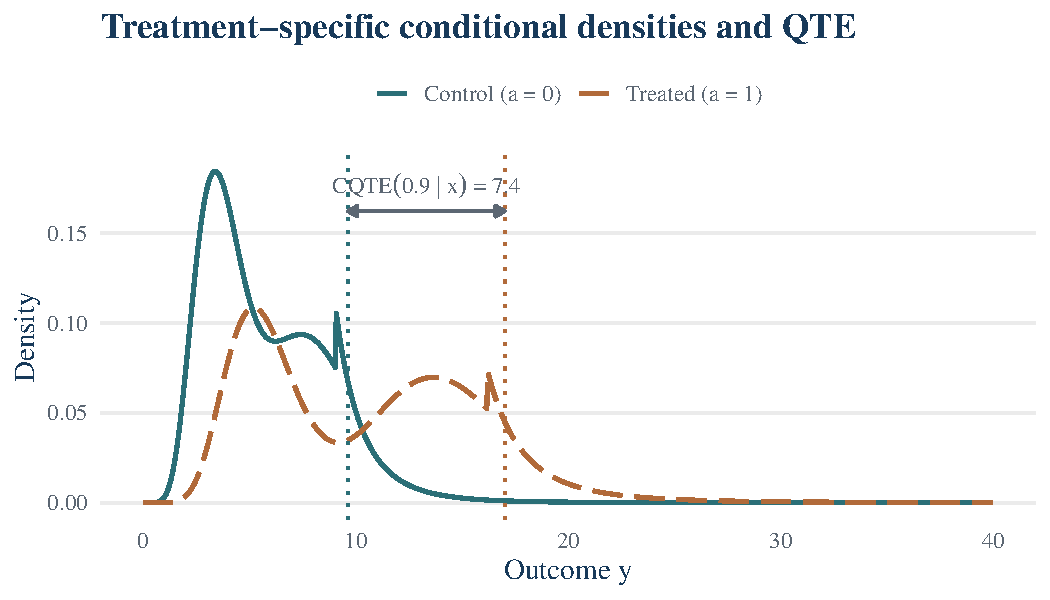
\includegraphics[width=0.78\linewidth]{figure/causalEstimandFigure-plot-1} 

}

\caption{Two arm-specific conditional outcome densities $f_a(y\mid x)$, $a\in\{0,1\}$, at a representative covariate profile $x$ under a spliced gamma-mixture-plus-GPD model: control arm ($a=0$, solid) and treated arm ($a=1$, long-dash). Dotted vertical lines mark the 90th conditional quantiles $Q_0(0.9\mid x)$ and $Q_1(0.9\mid x)$, and the double-headed arrow connects them, labelled with the conditional quantile treatment effect $\mathrm{CQTE}(0.9\mid x)=Q_1(0.9\mid x)-Q_0(0.9\mid x)$.}\label{fig:causalEstimandFigure-plot}
\end{figure}

\end{knitrout}

The package reports the causal estimands listed in
Table~\ref{tab:causal-estimands-main}, where superscripts
$\mathrm{m}$ and $\mathrm{t}$ denote full-population and
treated-population standardization, respectively.

\begin{table}[H]
\centering
\small
\caption[Causal estimands reported by the package]{Causal estimands reported by \pkg{CausalMixGPD}. Columns list the estimand name, its defining contrast as a functional of the treatment-specific outcome distributions, and the target population.}
\label{tab:causal-estimands-main}
{
\renewcommand{\arraystretch}{1.15}
\begin{tabular}{
  @{}>{\raggedright\arraybackslash}p{0.15\linewidth}
  >{\centering\arraybackslash}p{0.30\linewidth}
  >{\raggedright\arraybackslash}p{0.40\linewidth}@{}
}
\toprule
Estimand & Formula & Target population \\
\midrule
ATE & $\mu_1^{\mathrm{m}}-\mu_0^{\mathrm{m}}$ & Entire population \\
ATT & $\mu_1^{\mathrm{t}}-\mu_0^{\mathrm{t}}$ & Treated sub-population \\
QTE$(\tau)$ & $Q_1^{\mathrm{m}}(\tau)-Q_0^{\mathrm{m}}(\tau)$ & Entire population at index $\tau$\\
QTT$(\tau)$ & $Q_1^{\mathrm{t}}(\tau)-Q_0^{\mathrm{t}}(\tau)$ & Treated sub-population at index $\tau$\\
CATE$(x)$ & $\mu_1(x)-\mu_0(x)$ & Individual with covariate profile $x$ \\
CQTE$(\tau\mid x)$ & $Q_1(\tau\mid x)-Q_0(\tau\mid x)$ & Individual with $x$ at index $\tau$\\
\bottomrule
\end{tabular}
}
\end{table}

The next section describes how the package fits the treatment-specific
conditional distributions and computes these estimands from posterior
predictive output.


\section{Package Overview: Workflow, Model, and Inference}
\label{sec:overview}

This section describes the workflow for fitting conditional models and
obtaining predictions with \pkg{CausalMixGPD}.  The presentation
begins with the one-arm setup, in which the spliced DPM--GPD model is
fitted to an outcome conditional on covariates. The causal extension augments this
framework with arm-specific outcome models and an optional propensity
score augmentation for observational studies.
Simulated data sets bundled with the package are used throughout to
illustrate the main features; these are accessible via
\code{data()}.

\subsection{Spliced Regression model, Likelihood, and Covariate Dependence}
\label{subsec:overview-model}

The observed data consist of $n$ outcome--covariate pairs
$\mathcal{D}=\{(y_i,x_i)\}_{i=1}^n$, where $x_i\in\mathbb{R}^p$
denotes the covariate vector for unit $i$, optionally including an
intercept column.

\begin{knitrout}\footnotesize
\definecolor{shadecolor}{rgb}{0.969, 0.969, 0.969}\color{fgcolor}\begin{kframe}
\begin{alltt}
\hlkwd{data}\hldef{(}\hlsng{"nc_posX100_p3_k2"}\hldef{,} \hlkwc{package} \hldef{=} \hlsng{"CausalMixGPD"}\hldef{)}
\hldef{dat} \hlkwb{<-} \hlkwd{data.frame}\hldef{(}\hlkwc{y} \hldef{= nc_posX100_p3_k2}\hlopt{$}\hldef{y, nc_posX100_p3_k2}\hlopt{$}\hldef{X)}
\end{alltt}
\end{kframe}
\end{knitrout}

The conditional target distribution $F(\cdot\mid x)$ and the DPM--GPD
spliced construction are provided in Section~\ref{sec:prelim},
with the resulting spliced CDF and density functions given in
\eqref{eq:splice_cdf}--\eqref{eq:splice_pdf}. To perform posterior
inference, \pkg{CausalMixGPD} truncates the infinite mixture into
a finite DPM with $J$ components such that
\begin{equation*}
f_{\mathrm{DP}}(y\mid x;\Theta)\;\approx\;\sum_{j=1}^{J} w_j\,k(y\mid x;\theta_j),
\end{equation*}
where $j=1,\ldots,J$ indexes each mixture component, $w_j\ge 0$
are the corresponding mixture component weights, and the sum equals
one up to some residual probability mass allocated to other
components. Kernel parameters can be constant, specific to a
mixture component, or dependent on the covariates according to
link functions of the form
\begin{equation*}
  g\!\left(\psi_j(x)\right)=x^\top \beta_{j,\psi},
\end{equation*}
Here, $\psi_j(x)$ is a generic kernel parameter for component $j$
with input covariates $x$, while the link function $g(\cdot)$
restricts the parameter support. All code illustrations in this
section utilize the MCMC sampling options shown below;
longer sampling and multiple chains are encouraged in applied settings.

\begin{knitrout}\footnotesize
\definecolor{shadecolor}{rgb}{0.969, 0.969, 0.969}\color{fgcolor}\begin{kframe}
\begin{alltt}
\hlkwd{data.frame}\hldef{(mcmc_fixed,}\hlkwc{row.names} \hldef{=} \hlkwa{NULL}\hldef{)}
\end{alltt}
\begin{verbatim}
  niter nburnin thin nchains seed
1  2000     500    1       1 2026
\end{verbatim}
\end{kframe}
\end{knitrout}

The single-arm splicing approach can be performed by passing a
formula, data, and control options to \code{dpmgpd()}. The
\code{formula} argument uses standard \textsf{R} syntax to indicate
which covariates enter both the bulk and tail DPM components.
The \code{backend} option indicates whether the DPM component
weights should be represented using stick breaking in~\eqref{eq:sb}
or the Chinese restaurant process formulation. The \code{kernel}
argument selects the bulk mixture kernel, \code{components}
controls the number of components, and \code{mcmc} sets sampling

\begin{knitrout}\footnotesize
\definecolor{shadecolor}{rgb}{0.969, 0.969, 0.969}\color{fgcolor}\begin{kframe}
\begin{alltt}
\hldef{fit} \hlkwb{<-} \hlkwd{dpmgpd}\hldef{(}\hlkwc{formula} \hldef{= y} \hlopt{~} \hldef{x1} \hlopt{+} \hldef{x2} \hlopt{+} \hldef{x3,} \hlkwc{data} \hldef{= dat,} \hlkwc{mcmc} \hldef{= mcmc_fixed)}
\end{alltt}
\end{kframe}
\end{knitrout}

Given the spliced density in~\eqref{eq:splice_pdf}, the likelihood is given by
\begin{equation}
  L(\Theta,\Phi;\mathcal{D})
  =\prod_{i=1}^n f(y_i\mid x_i;\Theta,\Phi),
  \label{eq:overview-lik}
\end{equation}
where $\Theta$ collects the bulk parameters
$\{w_j,\theta_j\}_{j=1}^J$ and $\Phi$ collects the tail parameters
governing $u(x)$, $\sigma(x)$, and $\xi$.  The log-likelihood can
equivalently be written as
\begin{align*}
  \log L(\Theta,\Phi;\mathcal{D})
  \;=&\;\sum_{i=1}^n (1-\delta_i)\,\log f_{\mathrm{DP}}(y_i\mid x_i;\Theta)
  \\
  &\;+\;\sum_{i=1}^n \delta_i
  \Bigl[
    \log\!\bigl\{1-F_{\mathrm{DP}}(u(x_i)\mid x_i;\Theta)\bigr\}
    +\log f_{\mathrm{GPD}}\!\bigl(y_i\mid x_i;\Phi\bigr)
  \Bigr],
\end{align*}
where $f_{\mathrm{GPD}}$ is the GPD tail density from
Section~\ref{subsec:splice} and $F_{\mathrm{DP}}(\cdot\mid x)$ is the
bulk mixture CDF.

When the GPD tail is not included, the model reduces to
$f(y\mid x;\Theta, \Phi) \equiv f_{\text{DP}}(y \mid x; \Theta)$, a
mixture over the bulk alone.  A convenience interface to this bulk-only
model is provided by the \code{dpmix()} wrapper.

\begin{knitrout}\footnotesize
\definecolor{shadecolor}{rgb}{0.969, 0.969, 0.969}\color{fgcolor}\begin{kframe}
\begin{alltt}
\hldef{fit} \hlkwb{<-} \hlkwd{dpmix}\hldef{(}\hlkwc{formula} \hldef{= y} \hlopt{~} \hldef{x1} \hlopt{+} \hldef{x2} \hlopt{+} \hldef{x3,} \hlkwc{data} \hldef{= dat,} \hlkwc{mcmc} \hldef{= mcmc_fixed)}
\end{alltt}
\end{kframe}
\end{knitrout}

Prior distributions for $\Theta$ and $\Phi$ can be specified by the
user; defaults are weakly informative.  For the DPM parameters
$\Theta$, the default prior employs stick-breaking priors for the
mixture weights and conjugate priors for kernel parameters when
conjugacy obtains.  For the tail parameters $\Phi$, the default adopts
a regression-based specification for the threshold $u(x)$ and scale
$\sigma(x)$, together with a weakly informative prior for the shape
parameter~$\xi$.

\subsection{Statistical Inference: Estimation and prediction}
\label{subsec:overview-mcmc}

Posterior simulation targets the joint posterior, which is given by
$$p(\Theta,\Phi\mid \mathcal{D}) \propto L(\Theta,\Phi;\mathcal{D})\,p(\Theta,\Phi)$$
using the likelihood~\eqref{eq:overview-lik} and the prior structure
described in Section~\ref{subsec:overview-model}.
\pkg{CausalMixGPD} conducts MCMC via \pkg{nimble}
\citep{nimble_pkg}.  The fitted object supports \code{summary()} for
posterior summaries, \code{plot()} for standard MCMC diagnostics, and
\code{params()} for lightweight parameter extraction.

\begin{knitrout}\footnotesize
\definecolor{shadecolor}{rgb}{0.969, 0.969, 0.969}\color{fgcolor}\begin{kframe}
\begin{alltt}
\hlkwd{summary}\hldef{(fit)}  \hlcom{# posterior summaries for parameters and functionals}
\hlkwd{params}\hldef{(fit)}   \hlcom{# extract MCMC samples for parameters and functionals}
\hlkwd{plot}\hldef{(fit,} \hlkwc{family} \hldef{=} \hlsng{"traceplot"}\hldef{,} \hlkwc{params} \hldef{=} \hlsng{"alpha"}\hldef{)} \hlcom{# traceplot for concentration parameter}
\hlkwd{plot}\hldef{(fit,} \hlkwc{family} \hldef{=} \hlsng{"auto"}\hldef{)} \hlcom{# automatic selection of diagnostic plots for all parameters}
\end{alltt}
\end{kframe}
\end{knitrout}

The package provides posterior summaries for several functionals of the
fitted conditional distribution defined in
Section~\ref{sec:prelim}: the density $f(y\mid x)$, survival function
$S(y\mid x) = 1 - F(y\mid x)$, quantile function $Q(\tau\mid x)$,
and mean $\mathrm{E}(y\mid x)$.  For the \code{density},
\code{survival}, and \code{quantile} types, each functional is
evaluated draw-by-draw from
\eqref{eq:splice_cdf}--\eqref{eq:splice_quantile_case}, and the
retained draws are then summarized.  For \code{type = "mean"}, the
package employs analytical draw-level calculations whenever the kernel
mean exists and, for spliced GPD models, the tail-shape parameter
satisfies $\xi < 1$; if these conditions are not met, the ordinary
mean is not reported and the user is directed to
\code{type = "rmean"}.  The restricted-mean target
(\code{type = "rmean"}) provides a separate posterior predictive Monte
Carlo calculation for a user-supplied cutoff and remains well-defined
even when the ordinary mean does not exist.  The following code
illustrates how posterior density, quantile, and mean summaries are
obtained at observed covariate values, together with credible intervals
for quantiles and HPD intervals for means.

\begin{knitrout}\footnotesize
\definecolor{shadecolor}{rgb}{0.969, 0.969, 0.969}\color{fgcolor}\begin{kframe}
\begin{alltt}
\hlkwd{predict}\hldef{(fit,} \hlkwc{type} \hldef{=} \hlsng{"density"}\hldef{,} \hlkwc{interval} \hldef{=} \hlsng{"credible"}\hldef{,} \hlkwc{level} \hldef{=} \hlnum{0.95}\hldef{)}
\hlkwd{predict}\hldef{(fit,} \hlkwc{type} \hldef{=} \hlsng{"quantile"}\hldef{,} \hlkwc{index} \hldef{=} \hlkwd{c}\hldef{(}\hlnum{0.25}\hldef{,} \hlnum{0.5}\hldef{,} \hlnum{0.75}\hldef{))}
\hlkwd{predict}\hldef{(fit,} \hlkwc{type} \hldef{=} \hlsng{"mean"}\hldef{,} \hlkwc{interval} \hldef{=} \hlsng{"hpd"}\hldef{,} \hlkwc{level} \hldef{=} \hlnum{0.9}\hldef{)}
\end{alltt}
\end{kframe}
\end{knitrout}

Predictions at new covariate values are obtained by calling
\code{predict()} with a data set or covariate profiles sharing the
same structure as the training data.

\begin{knitrout}\footnotesize
\definecolor{shadecolor}{rgb}{0.969, 0.969, 0.969}\color{fgcolor}\begin{kframe}
\begin{alltt}
\hldef{x_new} \hlkwb{<-} \hlkwd{as.data.frame}\hldef{(}\hlkwd{lapply}\hldef{(dat[,} \hlkwd{c}\hldef{(}\hlsng{"x1"}\hldef{,} \hlsng{"x2"}\hldef{,} \hlsng{"x3"}\hldef{)], quantile,}
                              \hlkwc{probs} \hldef{=} \hlkwd{c}\hldef{(}\hlnum{0.25}\hldef{,} \hlnum{0.50}\hldef{,} \hlnum{0.75}\hldef{),} \hlkwc{na.rm} \hldef{=} \hlnum{TRUE}\hldef{))}
\hldef{y_grid} \hlkwb{<-} \hlkwd{seq}\hldef{(}\hlnum{0}\hldef{,} \hlnum{10}\hldef{,} \hlkwc{length.out} \hldef{=} \hlnum{200}\hldef{)}
\end{alltt}
\end{kframe}
\end{knitrout}

For a covariate profile $\boldsymbol{x}^\star$, predictions are obtained from the
posterior predictive density
\begin{equation*}
p(y^\star\mid \boldsymbol{x}^\star, \mathcal{D})
=\int f(y^\star\mid \boldsymbol{x}^\star; \Theta, \Phi)\,p(\Theta, \Phi\mid \mathcal{D})\,d\Theta\,d\Phi.
\end{equation*}
Predictions of the density and survival functions involve a grid of $y$
values provided through the \code{y} argument, while predictions of quantiles
require only the probability indices through the \code{index} argument.
The code example that follows provides posterior survival and quantile
predictions for new covariate profiles derived from the empirical
quartiles of the predictors in the training data.

The argument-level controls for the above methods are provided in
Appendix~\ref{sec:appendix-features}. Specifically,
Section~\ref{subsec:app-modeling} extends the prior and backend
definitions discussed previously, whereas Section~\ref{subsec:app-fitting} summarizes the full prediction,
interval, and diagnostic interfaces.

\begin{knitrout}\footnotesize
\definecolor{shadecolor}{rgb}{0.969, 0.969, 0.969}\color{fgcolor}\begin{kframe}
\begin{alltt}
\hlkwd{predict}\hldef{(fit,} \hlkwc{newdata} \hldef{= x_new,} \hlkwc{y} \hldef{= y_grid,} \hlkwc{type} \hldef{=} \hlsng{"survival"}\hldef{,} \hlkwc{level} \hldef{=} \hlnum{0.95}\hldef{)}
\hlkwd{predict}\hldef{(fit,} \hlkwc{newdata} \hldef{= x_new,} \hlkwc{type} \hldef{=} \hlsng{"quantile"}\hldef{,} \hlkwc{index} \hldef{=} \hlkwd{c}\hldef{(}\hlnum{0.5}\hldef{,} \hlnum{0.99}\hldef{),} \hlkwc{interval} \hldef{=} \hlsng{"credible"}\hldef{)}
\end{alltt}
\end{kframe}
\end{knitrout}



\subsection{Clustering extension}
\label{subsec:cluster_extension}

\begin{knitrout}\footnotesize
\definecolor{shadecolor}{rgb}{0.969, 0.969, 0.969}\color{fgcolor}\begin{kframe}
\begin{alltt}
\hlkwd{data}\hldef{(}\hlsng{"nc_realX100_p3_k2"}\hldef{,} \hlkwc{package} \hldef{=} \hlsng{"CausalMixGPD"}\hldef{)}
\hldef{dat_cl} \hlkwb{<-} \hlkwd{data.frame}\hldef{(}\hlkwc{y} \hldef{= nc_realX100_p3_k2}\hlopt{$}\hldef{y[}\hlnum{1}\hlopt{:}\hlnum{100}\hldef{], nc_realX100_p3_k2}\hlopt{$}\hldef{X[}\hlnum{1}\hlopt{:}\hlnum{100}\hldef{, ])}
\end{alltt}
\end{kframe}
\end{knitrout}
Under the clustering approach, the fitted mixture is regarded as a latent partition, and the output is cluster summaries.  For a mixture model without the optional GPD tail, the function \code{dpmix.cluster()} is called to perform clustering; otherwise, \code{dpmgpd.cluster()} is used, with predictor dependence introduced via weights, mixture parameters, or both.  Since labels assigned to components are arbitrary, the primary results include label-free summaries of the fitted mixture, namely the posterior similarity matrix (PSM), the representative partition, the number of clusters, and the cluster assignment scores
\citep{Binder1978,Dahl2006}.  The same prediction interface \code{predict()} can produce cluster labels for training observations or assign clusters to new observations.

The code block below demonstrates how to fit a clustering model with covariates affecting mixture parameters, by setting \code{type = "param"}.

\begin{knitrout}\footnotesize
\definecolor{shadecolor}{rgb}{0.969, 0.969, 0.969}\color{fgcolor}\begin{kframe}
\begin{alltt}
\hldef{fit_cluster} \hlkwb{<-} \hlkwd{dpmix.cluster}\hldef{(y} \hlopt{~} \hldef{x1} \hlopt{+} \hldef{x2} \hlopt{+} \hldef{x3,} \hlkwc{data} \hldef{= dat_cl[}\hlnum{1}\hlopt{:}\hlnum{100}\hldef{,],} \hlkwc{kernel} \hldef{=} \hlsng{"laplace"}\hldef{,}
                                  \hlkwc{type} \hldef{=} \hlsng{"both"}\hldef{,} \hlkwc{components} \hldef{=} \hlnum{10}\hldef{,} \hlkwc{mcmc} \hldef{= mcmc_fixed)}
\end{alltt}
\end{kframe}
\end{knitrout}

The function \code{predict()} accepts two types of predictions: posterior similarity matrix or cluster labels, determined by the \code{type} argument.

\begin{knitrout}\footnotesize
\definecolor{shadecolor}{rgb}{0.969, 0.969, 0.969}\color{fgcolor}\begin{kframe}
\begin{alltt}
\hlkwd{predict}\hldef{(fit_cluster,} \hlkwc{type} \hldef{=} \hlsng{"psm"}\hldef{)}
\end{alltt}
\end{kframe}
\end{knitrout}

Cluster labels of new observations, along with corresponding assignment scores, are calculated as follows.

\begin{knitrout}\footnotesize
\definecolor{shadecolor}{rgb}{0.969, 0.969, 0.969}\color{fgcolor}\begin{kframe}
\begin{alltt}
\hlkwd{predict}\hldef{(fit_cluster,} \hlkwc{newdata} \hldef{= dat_cl[}\hlnum{101}\hlopt{:}\hlnum{110}\hldef{,],} \hlkwc{type} \hldef{=} \hlsng{"label"}\hldef{)}
\end{alltt}
\end{kframe}
\end{knitrout}

In Section~\ref{subsec:clustering-theory}, we mentioned that the software supports three types of dependence and evaluates clustering performance based on PSM summaries and representative partitions.
Clustering-specific arguments and plotting options are described in Appendix~\ref{subsec:app-workflows}.



\subsection{Causal extension and propensity score augmentation}
\label{subsec:overview-causal}

The causal inference workflow consists of estimating the causal
framework separately per treatment arm and optionally augmenting the
outcome covariates with a summary of the propensity score (PS). In the
latter case (e.g., observational study), treatment allocation is
assumed to be Bernoulli distributed, as follows,
\begin{equation*}
A_i \mid \boldsymbol{x}_i \sim \mathrm{Bernoulli}\big(e_{\boldsymbol{\gamma}}(\boldsymbol{x}_i)\big),
\end{equation*}
and the predicted PS is included into the covariate vector to form an
augmented regressor,
\begin{equation*}
\boldsymbol{r}(\boldsymbol{x}) = \big(\boldsymbol{x}^\top,\ \psi\big(\widehat e(\boldsymbol{x})\big)\big)^\top,
\end{equation*}
where the PS link function (logit or probit) is determined by the
\code{PS} parameter and the transformation $\psi(\cdot)$ used on the
estimated propensity score depends on \code{ps\_scale}; the default
is the identity. Then, the outcome model in each arm is specified as
a spliced DPM-GPD regression in the augmented covariates; the
structure of splicing mixture regression is identical to that of
Section~\ref{subsec:overview-model}. In the setting of randomized
experiment, no PS estimation is needed, and the causal inference model
for each arm uses the exact same modeling workflow as in the
one-arm problem.

The code chunk below loads the data set generated from a benchmark
setup and constructs the input \code{data.frame} required by the
causal estimation workflows, consisting of the outcome, treatment
variable, and covariates.



The invocation of \code{dpmgpd.causal()} trains spliced mixture
regression for each treatment arm, with the causal model having the
same structure as \code{dpmgpd()} but taking into account additional
parameters controlling the PS model (\code{PS}, \code{ps\_scale},
\code{ps\_summary}) and different MCMC sampling strategies for the
outcome and PS components (\code{mcmc\_outcome}, \code{mcmc\_ps}).

\begin{knitrout}\footnotesize
\definecolor{shadecolor}{rgb}{0.969, 0.969, 0.969}\color{fgcolor}\begin{kframe}
\begin{alltt}
\hldef{causal_fit} \hlkwb{<-} \hlkwd{dpmgpd.causal}\hldef{(}\hlkwc{formula} \hldef{= y} \hlopt{~} \hldef{x1} \hlopt{+} \hldef{x2} \hlopt{+} \hldef{x3,} \hlkwc{data} \hldef{= causal_df,} \hlkwc{treat} \hldef{=} \hlsng{"A"}\hldef{,}
                            \hlkwc{backend} \hldef{=} \hlsng{"crp"}\hldef{,} \hlkwc{kernel} \hldef{=} \hlsng{"laplace"}\hldef{,} \hlkwc{components} \hldef{=} \hlnum{5}\hldef{,}
                            \hlkwc{PS} \hldef{=} \hlsng{"logit"}\hldef{,} \hlkwc{ps_scale} \hldef{=} \hlsng{"logit"}\hldef{,} \hlkwc{ps_summary} \hldef{=} \hlsng{"mean"}\hldef{,}
                            \hlkwc{mcmc_outcome} \hldef{= mcmc_fixed,} \hlkwc{mcmc_ps} \hldef{= mcmc_fixed)}
\end{alltt}
\end{kframe}
\end{knitrout}

Estimated population-averaged quantities are computed using the
functions \code{ate()} and \code{qte()}, and counterparts with
treatment-population averaging are implemented through \code{att()}
and \code{qtt()}. Confidence intervals are supported through
interval estimation, and results can be visualized by invoking the
generic \code{plot()} function with \code{type="effect"}, which
plots estimated effects across quantiles along with the corresponding
uncertainty bounds. The below code snippet shows the use of
\code{qtt()} to compute treated population effects.

\begin{knitrout}\footnotesize
\definecolor{shadecolor}{rgb}{0.969, 0.969, 0.969}\color{fgcolor}\begin{kframe}
\begin{alltt}
\hldef{qtt} \hlkwb{<-} \hlkwd{qtt}\hldef{(causal_fit,} \hlkwc{probs} \hldef{=} \hlkwd{c}\hldef{(}\hlnum{0.50}\hldef{,} \hlnum{0.90}\hldef{,} \hlnum{0.95}\hldef{),} \hlkwc{interval} \hldef{=} \hlsng{"credible"}\hldef{)}
\hlkwd{summary}\hldef{(qtt)}
\hlkwd{plot}\hldef{(qtt,} \hlkwc{type} \hldef{=} \hlsng{"effect"}\hldef{)}
\end{alltt}
\end{kframe}
\end{knitrout}

Quantified conditional causal effects based on user-provided
covariate profiles can be evaluated by the generic
\code{predict()} function, which returns the selected summary of the
posterior predictive outcome distribution depending on the value of the \code{type}
parameter; the examples below produce survival probabilities at a
grid of user-defined covariate values covering the empirical quartiles
of the training variables.



\begin{knitrout}\footnotesize
\definecolor{shadecolor}{rgb}{0.969, 0.969, 0.969}\color{fgcolor}\begin{kframe}
\begin{alltt}
\hlkwd{predict}\hldef{(causal_fit,} \hlkwc{newdata} \hldef{= causal_xgrid,} \hlkwc{type} \hldef{=} \hlsng{"survival"}\hldef{,} \hlkwc{y} \hldef{=} \hlkwd{rep}\hldef{(}\hlnum{4}\hldef{,} \hlkwd{nrow}\hldef{(causal_xgrid)))}
\end{alltt}
\end{kframe}
\end{knitrout}
The corresponding bulk-only version is \code{dpmix.causal()},
where the causal estimand and prediction remain unchanged without
the GPD tail. For randomized trials, the procedure is identical but
without the PS adjustment, where \code{PS} can be set to \code{NULL}.
Other causal estimands, PS adjustments, and plots are documented in
Appendix~\ref{subsec:app-workflows}.


\section{Data Analysis~I: Clustering}
\label{sec:app-clustering}

This section demonstrates clustering under a bulk-only conditional mixture model. The goal is to discover latent subgroups among the observational units using the fitted mixture model, while accounting for partition uncertainty in a label-invariant manner. Unlike the density prediction focus of Section~\ref{sec:overview}, here the interest lies in partition summaries and cluster membership for out-of-sample data. Key outputs include the posterior similarity matrix (PSM), a representative partition, and cluster assignments for held-out observations.

\subsection{Data and preprocessing}

The Boston data set is used in this analysis, where each observation corresponds to a census tract. The response variable used is medv, representing median home prices in each area. Predictors used include the lstat, rm, and nox variables, which represent the level of neighborhood disadvantage, the size of the houses, and pollution levels, respectively. This combination of predictors constitutes a well-motivated choice for discovering representative clusters. We are interested in uncovering representative clusters from amongst the data, and predicting which latent clusters held-out census tracts belong to using out-of-sample prediction. An 80\%/20\% train-test split was conducted.

\begin{knitrout}\footnotesize
\definecolor{shadecolor}{rgb}{0.969, 0.969, 0.969}\color{fgcolor}\begin{kframe}
\begin{alltt}
\hlkwd{library}\hldef{(CausalMixGPD)}
\hlkwd{library}\hldef{(MASS)}

\hlkwd{set.seed}\hldef{(}\hlnum{123}\hldef{)}
\hlkwd{data}\hldef{(}\hlsng{"Boston"}\hldef{,} \hlkwc{package} \hldef{=} \hlsng{"MASS"}\hldef{)}

\hldef{dat} \hlkwb{<-} \hldef{Boston}
\hldef{dat} \hlkwb{<-} \hlkwd{subset}\hldef{(dat,} \hlkwc{select} \hldef{=} \hlkwd{c}\hldef{(medv, lstat, rm, nox))}

\hldef{n} \hlkwb{<-} \hlkwd{nrow}\hldef{(dat)}
\hldef{idx_train} \hlkwb{<-} \hlkwd{sample}\hldef{(}\hlkwd{seq_len}\hldef{(n),} \hlkwc{size} \hldef{=} \hlkwd{floor}\hldef{(}\hlnum{0.80} \hlopt{*} \hldef{n),} \hlkwc{replace} \hldef{=} \hlnum{FALSE}\hldef{)}
\hldef{train_dat} \hlkwb{<-} \hldef{dat[idx_train, ]}
\hldef{test_dat}  \hlkwb{<-} \hldef{dat[}\hlopt{-}\hldef{idx_train, ]}
\end{alltt}
\end{kframe}
\end{knitrout}
In Figure~\ref{fig:app_cluster_response_panels}, we show the descriptive analyses of the Boston housing price data as represented by the median home value (\code{medv}). The variability in the response is substantial, and the distribution exhibits a pronounced upper tail. A flexible mixture model is therefore better suited than a simple regression to capture this structure.

\begin{knitrout}\footnotesize
\definecolor{shadecolor}{rgb}{0.969, 0.969, 0.969}\color{fgcolor}\begin{figure}[H]

{\centering 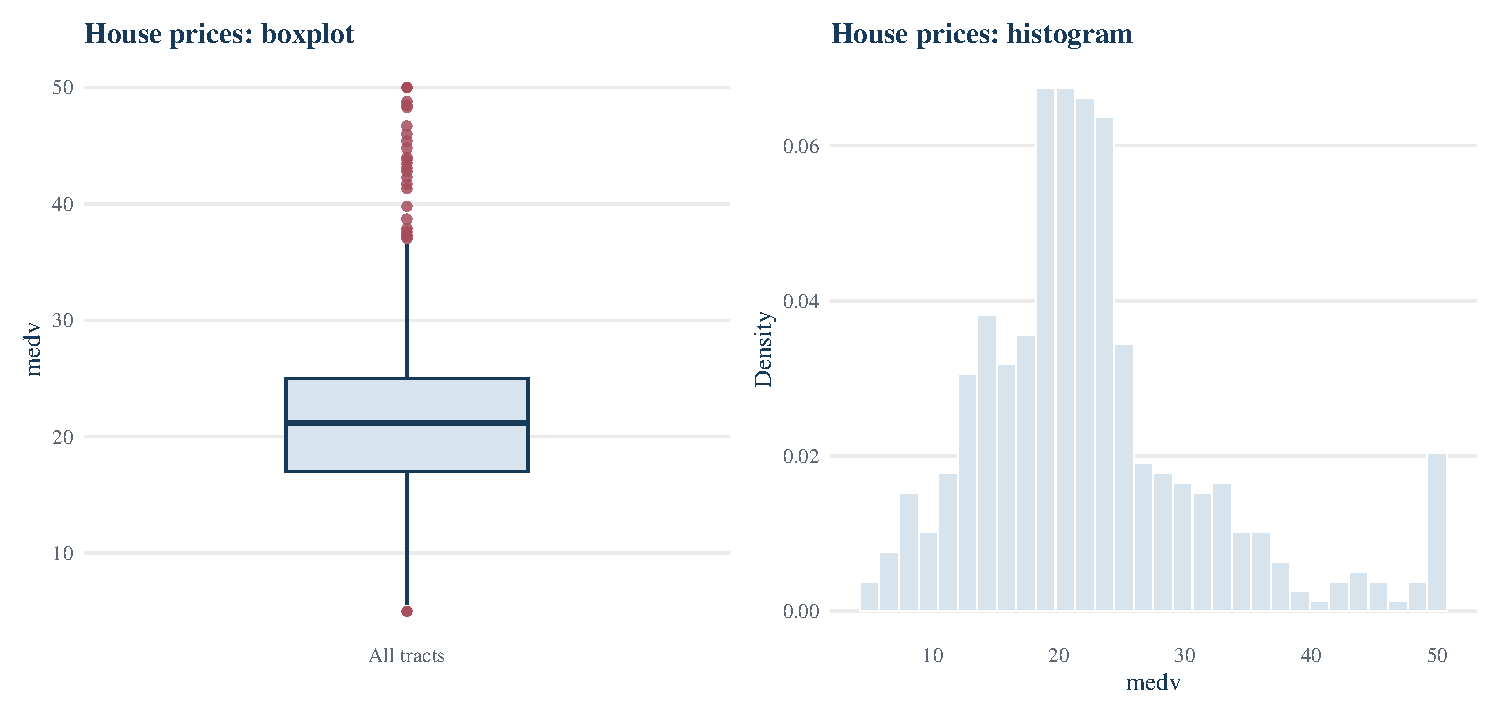
\includegraphics[width=0.95\linewidth]{figure/app_cluster_response_panels-1} 

}

\caption{Full-sample distribution of median house values (\code{medv}, in thousands of US dollars) for the $506$ census tracts in the \code{MASS::Boston} data set. Left panel: boxplot with upper outliers highlighted. Right panel: density-scaled histogram on the same variable.}\label{fig:app_cluster_response_panels}
\end{figure}

\end{knitrout}

\subsection{Model estimation and training cluster summaries}

A bulk only conditional mixture model is applied to the \code{medv}
dataset with three covariates. When \code{type = "weights"},
covariates determine the weights of the mixture while the parameters of the components are common across all covariates. This method is helpful for clustering where the prevalence of latent clusters may differ between neighborhoods.

\begin{knitrout}\footnotesize
\definecolor{shadecolor}{rgb}{0.969, 0.969, 0.969}\color{fgcolor}\begin{kframe}
\begin{alltt}
\hldef{fit_clust} \hlkwb{<-} \hlkwd{dpmix.cluster}\hldef{(} \hlkwc{formula} \hldef{= medv} \hlopt{~} \hldef{lstat} \hlopt{+} \hldef{rm} \hlopt{+} \hldef{nox,}
                              \hlkwc{data}  \hldef{= train_dat,} \hlkwc{kernel}   \hldef{=} \hlsng{"normal"}\hldef{,}
                               \hlkwc{type} \hldef{=} \hlsng{"weights"}\hldef{,} \hlkwc{components} \hldef{=} \hlnum{10}\hldef{,} \hlkwc{mcmc} \hldef{= mcmc_fixed)}
\end{alltt}
\end{kframe}
\end{knitrout}

Since mixture components cannot be identified up to permutation,
clusters in the training data are represented using the posterior
similarity matrix and sample training labels. The posterior similarity
matrix gives the main label-invariant uncertainty summary by
recording posterior co-clustering probabilities.

\begin{knitrout}\footnotesize
\definecolor{shadecolor}{rgb}{0.969, 0.969, 0.969}\color{fgcolor}\begin{kframe}
\begin{alltt}
\hldef{z_train_psm} \hlkwb{<-} \hlkwd{predict}\hldef{(fit_clust,} \hlkwc{type} \hldef{=} \hlsng{"psm"}\hldef{)}
\end{alltt}
\end{kframe}
\end{knitrout}

\begin{knitrout}\footnotesize
\definecolor{shadecolor}{rgb}{0.969, 0.969, 0.969}\color{fgcolor}\begin{kframe}
\begin{alltt}
\hlkwd{plot}\hldef{(z_train_psm,} \hlkwc{type} \hldef{=} \hlsng{"summary"}\hldef{)}
\end{alltt}
\end{kframe}\begin{figure}[H]

{\centering 
\includegraphics[width=0.85\linewidth]{figure/app_cluster_psm_plot-code-1} 

}

\caption{Posterior similarity matrix (PSM) summary for the Boston training sample, returned by \code{plot(predict(fit_clust, type = "psm"), type = "summary")}. Each cell $(i,\ell)$ encodes the posterior co-clustering probability $\Pr(z_i=z_\ell\mid\text{data})$, with rows and columns ordered to expose block structure. Darker shading corresponds to higher co-clustering probability.}\label{fig:app_cluster_psm_plot-code}
\end{figure}

\end{knitrout}

As seen from Figure~\ref{fig:app_cluster_psm_plot-code}, the PSM
reveals clear block structure along the diagonal, implying that the
model can detect multiple sets of tracts whose co-clustering
probability is relatively high. While there are clear separations,
there are still some uncertainties for those tracts on the edge of
two or more neighboring groups, which reflects reasonable posterior
uncertainty in a non-experimental housing dataset, since features of
neighborhoods tend to change gradually rather than abruptly.

\begin{knitrout}\footnotesize
\definecolor{shadecolor}{rgb}{0.969, 0.969, 0.969}\color{fgcolor}\begin{kframe}
\begin{alltt}
\hldef{z_train_lab} \hlkwb{<-} \hlkwd{predict}\hldef{(fit_clust,} \hlkwc{type} \hldef{=} \hlsng{"label"}\hldef{)}
\end{alltt}
\end{kframe}
\end{knitrout}

Figure~\ref{fig:app_cluster_overlay} shows the representative training
cluster summary produced by the package \code{plot()} method applied
to the training labels object.

\begin{knitrout}\footnotesize
\definecolor{shadecolor}{rgb}{0.969, 0.969, 0.969}\color{fgcolor}\begin{kframe}
\begin{alltt}
\hlkwd{plot}\hldef{(z_train_lab,} \hlkwc{type} \hldef{=} \hlsng{"summary"}\hldef{)}
\end{alltt}
\end{kframe}\begin{figure}[H]

{\centering 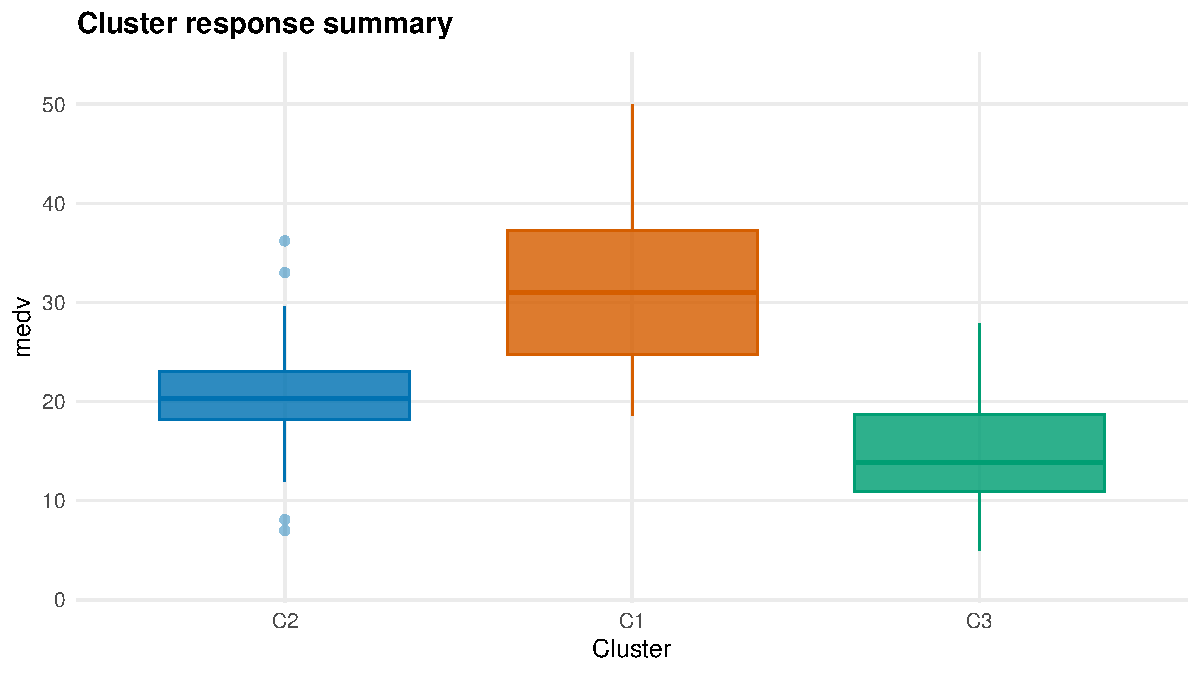
\includegraphics[width=0.85\linewidth]{figure/app_cluster_overlay-1} 

}

\caption[Representative training-cluster summary for the Boston \code{medv} analysis, returned by the \code{plot()} method applied to the labels object from \code{predict(fit_clust, type = "label")}]{Representative training-cluster summary for the Boston \code{medv} analysis, returned by the \code{plot()} method applied to the labels object from \code{predict(fit_clust, type = "label")}. Training observations are shown on the response scale and coloured by their assigned cluster in the representative partition.}\label{fig:app_cluster_overlay}
\end{figure}

\end{knitrout}

The representative partition translates the posterior co-clustering
structure into an interpretable summary on the response scale. The
inferred groups separate tracts primarily by housing-value level, but
they also reflect broader differences in neighborhood composition and
environmental quality. Thus, the clustering output is not merely a
numerical partition induced by the mixture fit; it yields a meaningful
summary of heterogeneity in the Boston housing data.

\subsection{Prediction for new observations}

Cluster assignment for new observations is performed through the same
prediction interface. The output is a label in the space of the
representative training clusters, obtained by aggregating posterior
predictive co-clustering evidence at the cluster level.

\begin{knitrout}\footnotesize
\definecolor{shadecolor}{rgb}{0.969, 0.969, 0.969}\color{fgcolor}\begin{kframe}
\begin{alltt}
\hldef{z_test} \hlkwb{<-} \hlkwd{predict}\hldef{( fit_clust,} \hlkwc{newdata} \hldef{= test_dat,} \hlkwc{type}    \hldef{=} \hlsng{"label"}\hldef{)}
\end{alltt}
\end{kframe}
\end{knitrout}

Figure~\ref{fig:app_cluster_test_sizes} displays the distribution of
predicted cluster assignments across the test sample, produced by the
package \code{plot()} method applied to the test labels object.

\begin{knitrout}\footnotesize
\definecolor{shadecolor}{rgb}{0.969, 0.969, 0.969}\color{fgcolor}\begin{kframe}
\begin{alltt}
\hlkwd{summary}\hldef{(z_test)}\hlopt{$}\hldef{cluster_profiles}
\end{alltt}
\begin{verbatim}
  cluster  n medv_mean  medv_sd lstat_mean lstat_sd
1      C4 53  21.57736 6.867192  13.415660 5.602698
2      C2 24  18.69583 5.343951  14.474583 7.229240
3      C5 18  35.15556 9.010988   5.679444 1.503887
4      C1  7  11.72857 2.293261  24.204286 6.162083
   rm_mean     rm_sd  nox_mean     nox_sd
1 6.225340 0.6417186 0.5775660 0.11813723
2 5.976583 0.4887950 0.5618333 0.12035912
3 7.260167 0.6143898 0.4957222 0.09672649
4 5.763571 0.5772723 0.6538571 0.09705227
\end{verbatim}
\end{kframe}
\end{knitrout}

\begin{knitrout}\footnotesize
\definecolor{shadecolor}{rgb}{0.969, 0.969, 0.969}\color{fgcolor}\begin{kframe}
\begin{alltt}
\hlkwd{plot}\hldef{(z_test,} \hlkwc{type} \hldef{=} \hlsng{"sizes"}\hldef{)}
\end{alltt}
\end{kframe}\begin{figure}[H]

{\centering 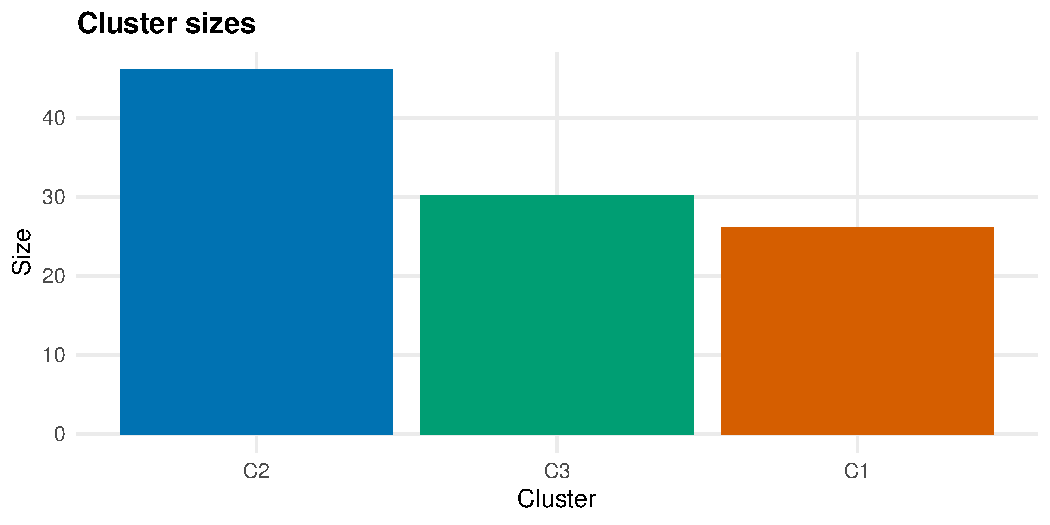
\includegraphics[width=0.8\linewidth]{figure/app_cluster_test_sizes-1} 

}

\caption{Bar plot of predicted cluster assignments for the held-out Boston test sample (the $20\%$ of \code{medv} observations excluded from training), returned by \code{plot(predict(fit_clust, newdata = test_dat, type = "label"), type = "sizes")}. Each bar corresponds to one representative training cluster from Figure~\ref{fig:app_cluster_overlay}; bar heights give the number of test tracts assigned to that cluster.}\label{fig:app_cluster_test_sizes}
\end{figure}

\end{knitrout}

The expected characteristics of the clusters' profiles are consistent with the interpretation of the representative partition. Cluster C5 contains the wealthiest tracts defined by a high mean house value, low average \code{lstat}, large mean number of rooms, and relatively low pollution. Cluster C1 represents the poorest neighborhoods with a low average house value, significant disadvantages in terms of neighborhood quality, low mean number of rooms, and a high level of pollution. Clusters C2 and C4 represent intermediate cases which show that multiple clusters were detected within the housing market rather than a bimodal distribution with poor and wealthy neighborhoods at its ends.

As expected, the vast majority of held-out tracts are classified into middle-value clusters (C4 and C2) with no tendency toward the low-end cluster. This is consistent with the Boston data, confirming that predictions are not unduly influenced by the outliers in the dataset. Tract assignments in the test set confirm the interpretation of the training-set partition: tracts belonging to more expensive clusters exhibit less neighborhood disadvantage, larger homes, and lower pollution, while tracts in poorer clusters exhibit the opposite characteristics.

This case study illustrates the workflow in which inference is summarized through a representative partition and cluster descriptions, and new observations are assigned to those clusters based on posterior predictive membership probabilities. The representative clusters also quantify the relationship between partition uncertainty and the marginal distributions of the response and covariates. The latent clusters align with the socioeconomic and environmental gradient, confirming that the nonparametric mixture recovers stable structure despite heterogeneity in the response. Causal comparisons are taken up in Section~\ref{sec:app-causal}.


\section{Data Analysis~II: Causal Inference}
\label{sec:app-causal}

This section describes the estimands from the two-arm spliced density regression. In contrast to the partition estimation of Section~\ref{sec:app-clustering}, the focus here is on mean and quantile differences for both unconditional and conditional causal estimands.

Data and estimands

To estimate unconditional and conditional causal estimands using the proposed approach, the \code{lalonde} dataset from the \pkg{MatchIt} \textsf{R} package is used for benchmarking. The outcome is the 1978 annual income level measured by \code{re78} (\$), and the treatment indicator corresponds to program participation (variable \code{treat}). Covariates include age, years of schooling, race, marriage status, college degree status, and prior earnings \code{re74} and \code{re75}. Earnings typically exhibit considerable skewness, concentrate near zero, and have a pronounced upper tail, motivating the use of quantile and tail summaries rather than the mean alone.

The four estimands in Table~\ref{tab:causal-estimands-main} are computed following Section~\ref{subsec:causal}. Standardized estimands (ATE, QTE) are averaged across the empirical distribution of \(\{\boldsymbol{x}_i\}_{i=1}^n\), while conditional estimands (CATE, CQTE) are evaluated at selected covariate profiles.

The data are first loaded and the design matrix constructed.

\begin{knitrout}\footnotesize
\definecolor{shadecolor}{rgb}{0.969, 0.969, 0.969}\color{fgcolor}\begin{kframe}
\begin{alltt}
\hlkwd{data}\hldef{(}\hlsng{"lalonde"}\hldef{,} \hlkwc{package} \hldef{=} \hlsng{"MatchIt"}\hldef{)}
\hldef{app_lalonde_covars} \hlkwb{<-} \hlkwd{within}\hldef{(lalonde, \{}
  \hldef{race} \hlkwb{<-} \hlkwd{factor}\hldef{(race,} \hlkwc{levels} \hldef{=} \hlkwd{c}\hldef{(}\hlsng{"white"}\hldef{,} \hlsng{"black"}\hldef{,} \hlsng{"hispan"}\hldef{))}
  \hldef{married} \hlkwb{<-} \hlkwd{factor}\hldef{(married,} \hlkwc{levels} \hldef{=} \hlkwd{c}\hldef{(}\hlnum{0}\hldef{,} \hlnum{1}\hldef{),} \hlkwc{labels} \hldef{=} \hlkwd{c}\hldef{(}\hlsng{"no"}\hldef{,} \hlsng{"yes"}\hldef{))}
  \hldef{nodegree} \hlkwb{<-} \hlkwd{factor}\hldef{(nodegree,} \hlkwc{levels} \hldef{=} \hlkwd{c}\hldef{(}\hlnum{0}\hldef{,} \hlnum{1}\hldef{),} \hlkwc{labels} \hldef{=} \hlkwd{c}\hldef{(}\hlsng{"no"}\hldef{,} \hlsng{"yes"}\hldef{))}
\hldef{\})}
\hldef{app_lalonde_scale_vars} \hlkwb{<-} \hlkwd{c}\hldef{(}\hlsng{"age"}\hldef{,} \hlsng{"educ"}\hldef{,} \hlsng{"re74"}\hldef{,} \hlsng{"re75"}\hldef{)}
\hldef{app_lalonde_scale_center} \hlkwb{<-} \hlkwd{vapply}\hldef{(}
  \hldef{app_lalonde_scale_vars,}
  \hlkwa{function}\hldef{(}\hlkwc{v}\hldef{)} \hlkwd{mean}\hldef{(app_lalonde_covars[[v]],} \hlkwc{na.rm} \hldef{=} \hlnum{TRUE}\hldef{),}
  \hlkwd{numeric}\hldef{(}\hlnum{1}\hldef{)}
\hldef{)}
\hldef{app_lalonde_scale_scale} \hlkwb{<-} \hlkwd{vapply}\hldef{(}
  \hldef{app_lalonde_scale_vars,}
  \hlkwa{function}\hldef{(}\hlkwc{v}\hldef{) stats}\hlopt{::}\hlkwd{sd}\hldef{(app_lalonde_covars[[v]],} \hlkwc{na.rm} \hldef{=} \hlnum{TRUE}\hldef{),}
  \hlkwd{numeric}\hldef{(}\hlnum{1}\hldef{)}
\hldef{)}
\hlkwa{for} \hldef{(v} \hlkwa{in} \hldef{app_lalonde_scale_vars) \{}
  \hldef{app_lalonde_covars[[}\hlkwd{paste0}\hldef{(v,} \hlsng{"_z"}\hldef{)]]} \hlkwb{<-}
    \hldef{(app_lalonde_covars[[v]]} \hlopt{-} \hldef{app_lalonde_scale_center[[v]])} \hlopt{/}
    \hldef{app_lalonde_scale_scale[[v]]}
\hldef{\}}
\hldef{app_lalonde_x_formula} \hlkwb{<-} \hlopt{~} \hldef{age_z} \hlopt{+} \hldef{educ_z} \hlopt{+} \hldef{race} \hlopt{+} \hldef{married} \hlopt{+} \hldef{nodegree} \hlopt{+} \hldef{re74_z} \hlopt{+} \hldef{re75_z}
\hldef{app_lalonde_y} \hlkwb{<-} \hldef{(app_lalonde_covars}\hlopt{$}\hldef{re78} \hlopt{+} \hlnum{0.5}\hldef{)} \hlopt{/} \hlnum{1000}
\hldef{app_lalonde_A} \hlkwb{<-} \hlkwd{as.integer}\hldef{(app_lalonde_covars}\hlopt{$}\hldef{treat)}
\hldef{app_lalonde_taus} \hlkwb{<-} \hlkwd{c}\hldef{(}\hlnum{0.25}\hldef{,} \hlnum{0.50}\hldef{,} \hlnum{0.75}\hldef{,} \hlnum{0.90}\hldef{,} \hlnum{0.95}\hldef{)}
\hldef{app_lalonde_X} \hlkwb{<-} \hldef{stats}\hlopt{::}\hlkwd{model.matrix}\hldef{(app_lalonde_x_formula,} \hlkwc{data} \hldef{= app_lalonde_covars}
                                                  \hldef{)[,} \hlopt{-}\hlnum{1}\hldef{,} \hlkwc{drop} \hldef{=} \hlnum{FALSE}\hldef{]}
\end{alltt}
\end{kframe}
\end{knitrout}

Figure~\ref{fig:app_lalonde_response_panels} provides full-sample
descriptive views of observed 1978 earnings (\code{re78}) by treatment
assignment. Both groups exhibit substantial mass near zero together
with pronounced right-skewness, and the arm-specific distributions
differ in ways that are not well summarized by a simple location shift.
These features motivate modeling the full treatment-specific outcome
distributions directly rather than relying solely on average effects.

\begin{knitrout}\footnotesize
\definecolor{shadecolor}{rgb}{0.969, 0.969, 0.969}\color{fgcolor}\begin{figure}[H]

{\centering 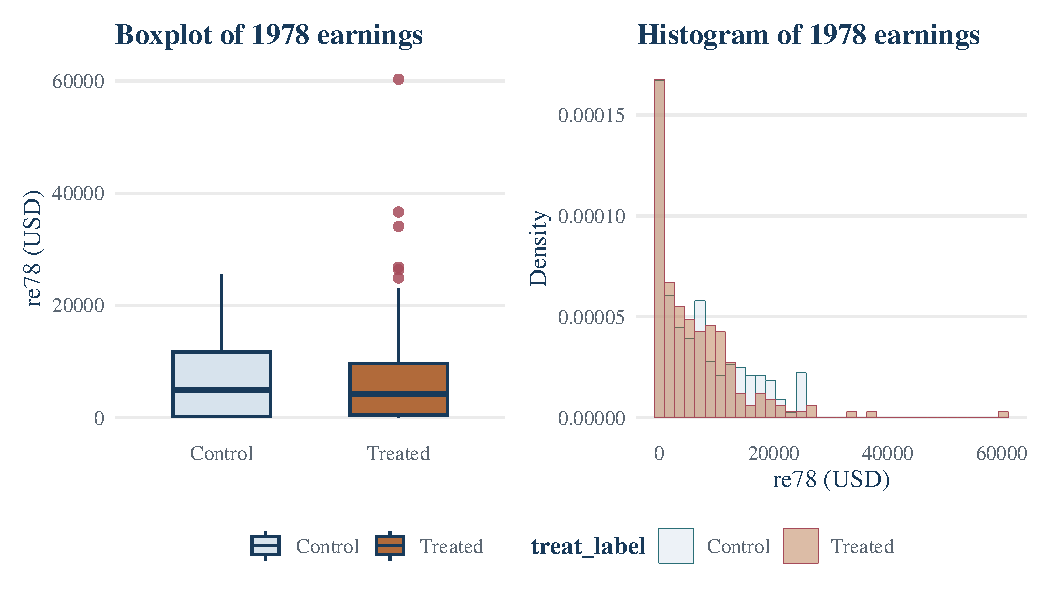
\includegraphics[width=0.95\linewidth]{figure/app_lalonde_response_panels-1} 

}

\caption{Full-sample distribution of 1978 annual earnings (\code{re78}, in US dollars) from the \code{MatchIt::lalonde} data set, stratified by treatment arm. Left panel: arm-specific boxplots with upper outliers highlighted. Right panel: overlaid density-scaled histograms for the control and treated arms.}\label{fig:app_lalonde_response_panels}
\end{figure}

\end{knitrout}

\subsection{Model and fit}

Arm-specific conditional outcome distributions
$F_a(\cdot\mid \boldsymbol{x})$ are modeled via the spliced bulk--tail
construction described in Section~\ref{subsec:splice}:
\begin{equation*}
f_a(y\mid \boldsymbol{x})
=
\sum_j w_{aj}(\boldsymbol{x})\, k(y\mid \Theta_{aj})\,\mathbf{1}(y\le u)
+
\{1-F_a(u\mid \boldsymbol{x})\}\, g(y\mid u,\sigma_a,\xi_a)\,\mathbf{1}(y>u).
\end{equation*}
The bulk kernel $k(\cdot)$ represents a Dirichlet process mixture
regression with a Chinese restaurant process backbone, while the tail
density $g(\cdot)$ follows the GPD distribution with positive scale
$\sigma_a>0$ and tail index $\xi_a$. In our model, the GPD tail index
$\xi_a$ regulates tail heaviness (e.g., if $\xi_a>0$, it indicates a
heavier tail). Our model mitigates poor finite-sample precision for extreme
quantiles through nonparametric bulk and EVT-consistent tail modeling.

Here, a two-sample mixture is fitted with the gamma bulk kernel and the
same MCMC configuration throughout. The aim is not to draw definitive
conclusions but to demonstrate how the package produces standardized and
conditional earnings contrasts under the spliced DPM-GPD framework.

\begin{knitrout}\footnotesize
\definecolor{shadecolor}{rgb}{0.969, 0.969, 0.969}\color{fgcolor}\begin{kframe}
\begin{alltt}
\hldef{fit} \hlkwb{<-} \hlkwd{dpmgpd.causal}\hldef{(}\hlkwc{y} \hldef{= app_lalonde_y,} \hlkwc{X} \hldef{= app_lalonde_X,} \hlkwc{treat} \hldef{= app_lalonde_A,}
                      \hlkwc{backend} \hldef{=} \hlsng{"crp"}\hldef{,} \hlkwc{kernel} \hldef{=} \hlsng{"gamma"}\hldef{,} \hlkwc{components} \hldef{=} \hlnum{10}\hldef{,} \hlkwc{mcmc} \hldef{= mcmc_fixed)}
\end{alltt}
\end{kframe}
\end{knitrout}



\subsection{Posterior summaries}

The fitted causal object defines two arm-specific outcome distributions
from which all reported summaries are derived. The framework is therefore
not limited to a single regression coefficient or scalar contrast; mean,
quantile, and tail-sensitive causal estimands are all coherent functionals
of the same fitted posterior distribution.

\begin{knitrout}\footnotesize
\definecolor{shadecolor}{rgb}{0.969, 0.969, 0.969}\color{fgcolor}\begin{kframe}
\begin{verbatim}
  total    ps    con    trt parallel_arms
1 418.5 31.77 262.91 123.77         FALSE
\end{verbatim}
\end{kframe}
\end{knitrout}

\subsection{Standardized estimands: ATE and QTE}

The overall treatment effect is summarized with ATE and QTE.

\begin{knitrout}\footnotesize
\definecolor{shadecolor}{rgb}{0.969, 0.969, 0.969}\color{fgcolor}\begin{kframe}
\begin{alltt}
\hldef{ate_fit} \hlkwb{<-} \hlkwd{ate}\hldef{(fit,} \hlkwc{interval} \hldef{=} \hlsng{"hpd"}\hldef{,} \hlkwc{level} \hldef{=} \hlnum{0.95}\hldef{)}
\hlkwd{summary}\hldef{(ate_fit)}
\end{alltt}
\begin{verbatim}
ATE Summary
================================================== 
Prediction points: 1
Conditional: NO | PS used: YES
Interval: hpd

Model specification:
  Backend (trt/con): crp / crp
  Kernel (trt/con): gamma / gamma
  GPD tail (trt/con): YES / YES

ATE estimates:
 estimate  lower upper
   -0.766 -2.992 1.358
\end{verbatim}
\end{kframe}
\end{knitrout}

The posterior ATE estimate is negative on the scaled earnings scale,
but the corresponding interval includes zero. Thus, after averaging
over the empirical covariate distribution, the analysis does not
provide strong evidence of a uniform overall mean effect of the
training program. Mean-based summaries alone are therefore insufficient
to characterize the program effect in this application.

\begin{knitrout}\footnotesize
\definecolor{shadecolor}{rgb}{0.969, 0.969, 0.969}\color{fgcolor}\begin{kframe}
\begin{alltt}
\hldef{qte_fit} \hlkwb{<-} \hlkwd{qte}\hldef{(fit,} \hlkwc{probs} \hldef{=} \hlkwd{c}\hldef{(}\hlnum{0.25}\hldef{,} \hlnum{0.50}\hldef{,} \hlnum{0.75}\hldef{),} \hlkwc{interval} \hldef{=} \hlsng{"credible"}\hldef{)}
\end{alltt}
\end{kframe}
\end{knitrout}

Figure~\ref{fig:qte_plot} displays two standardized QTE views side by
side from the spliced causal model: the effect curve and the
treated-versus-control quantile curves with uncertainty intervals.

\begin{knitrout}\footnotesize
\definecolor{shadecolor}{rgb}{0.969, 0.969, 0.969}\color{fgcolor}\begin{kframe}
\begin{alltt}
\hldef{qte_effect_plot} \hlkwb{<-} \hlkwd{plot}\hldef{(qte_fit,} \hlkwc{type} \hldef{=} \hlsng{"effect"}\hldef{)}
\hldef{qte_arms_plot} \hlkwb{<-} \hlkwd{plot}\hldef{(qte_fit,} \hlkwc{type} \hldef{=} \hlsng{"arms"}\hldef{)}
\hldef{qte_effect_plot} \hlopt{+} \hldef{qte_arms_plot} \hlopt{+} \hlkwd{plot_layout}\hldef{(}\hlkwc{ncol} \hldef{=} \hlnum{2}\hldef{)}
\end{alltt}
\end{kframe}\begin{figure}[H]

{\centering 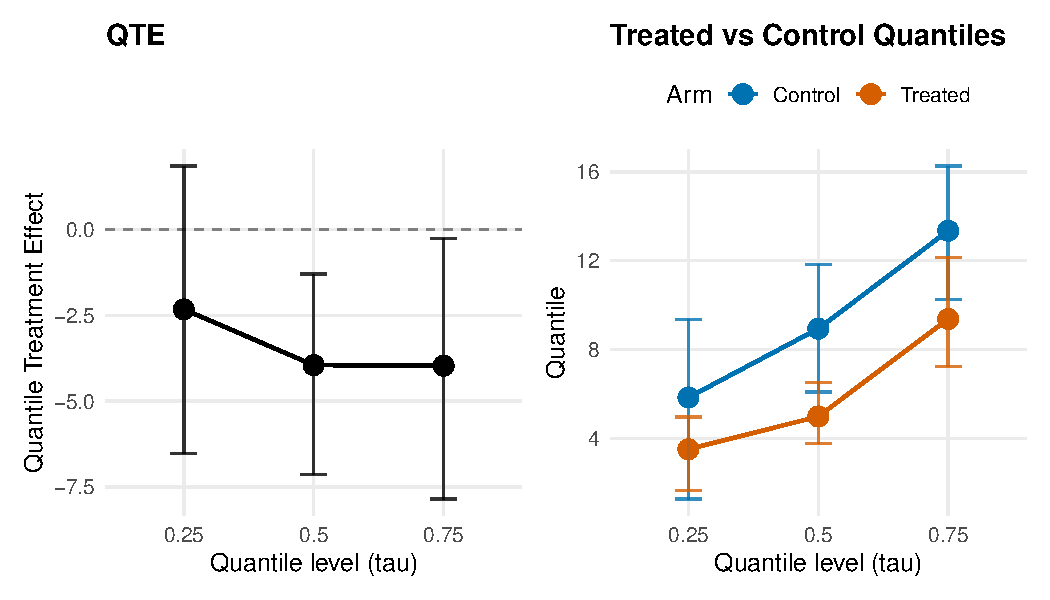
\includegraphics[width=0.95\linewidth]{figure/qte_plot-1} 

}

\caption{Standardized quantile treatment effect (QTE) summaries for Lalonde 1978 earnings, returned by \code{qte(fit, probs = c(0.25, 0.50, 0.75), interval = "credible")}. Left panel: effect curve $Q_1^{\mathrm{m}}(\tau)-Q_0^{\mathrm{m}}(\tau)$ versus $\tau$ with pointwise $95\%$ credible band. Right panel: standardized treated and control quantile curves $Q_1^{\mathrm{m}}(\tau)$ and $Q_0^{\mathrm{m}}(\tau)$ on the original earnings scale, with pointwise credible bands.}\label{fig:qte_plot}
\end{figure}

\end{knitrout}

The QTEs remain negative at the specified quantile levels, indicating that the treatment distribution lies below the control at those points of the marginal distribution. The marginal quantile curves for both arms show that the deviations are not reducible to a location shift but reflect heterogeneity across the outcome distribution.

\subsection{Conditional estimands for representative profiles}

To characterize heterogeneity in the treatment effect, conditional estimands are computed at four representative covariate profiles spanning the observed covariate range. Profile values are expressed on the original data scale, using empirical quantiles for continuous variables and observed levels for categorical variables. Continuous predictors are standardized using training-set means and standard deviations before being passed to the model.



\begin{table}[H]
\centering
\caption{\label{tab:xnew-results}Representative Lalonde participant profiles used as new-data inputs for the conditional causal contrasts in Figure~\ref{fig:cate_plot}. Columns (Profile~1--Profile~4) give the covariate values for one synthetic individual on the original data scale: \code{age} (years), \code{educ} (years of schooling), \code{race}, \code{married}, \code{nodegree}, and prior annual earnings \code{re74} and \code{re75} (US dollars).}
\centering
\resizebox{\ifdim\width>\linewidth\linewidth\else\width\fi}{!}{
\fontsize{8}{10}\selectfont
\begin{tabular}[t]{lllll}
\toprule
  & Profile 1 & Profile 2 & Profile 3 & Profile 4\\
\midrule
age & 20.0000 & 25.0000 & 32.0000 & 43.0000\\
educ & 9.0000 & 11.0000 & 12.0000 & 13.0000\\
race & black & hispan & white & black\\
married & no & no & yes & yes\\
nodegree & yes & no & no & yes\\
\addlinespace
re74 & 0.0000 & 47.4143 & 2705.7476 & 9383.2356\\
re75 & 0.0000 & 16.4710 & 1389.6486 & 4201.8870\\
\bottomrule
\end{tabular}}
\end{table}



\begin{knitrout}\footnotesize
\definecolor{shadecolor}{rgb}{0.969, 0.969, 0.969}\color{fgcolor}\begin{kframe}
\begin{alltt}
\hldef{cate_fit} \hlkwb{<-} \hlkwd{cate}\hldef{(fit,} \hlkwc{newdata} \hldef{= xnew,} \hlkwc{interval} \hldef{=} \hlsng{"hpd"}\hldef{,} \hlkwc{show_progress} \hldef{=} \hlnum{FALSE}\hldef{)}
\hlkwd{summary}\hldef{(cate_fit)}
\hlcom{# plot(cate_fit, type = "effect") # Displays mean-based CATE plot by profile}
\end{alltt}
\end{kframe}
\end{knitrout}

The mean-based conditional average treatment effects are generally
modest and uncertain. Although some profiles show positive point
estimates, the corresponding intervals are broad and typically overlap
zero. Thus, at the level of conditional means, the program does not
appear to induce a strong and uniform shift in earnings across all
participant types.

\begin{knitrout}\footnotesize
\definecolor{shadecolor}{rgb}{0.969, 0.969, 0.969}\color{fgcolor}\begin{kframe}
\begin{alltt}
\hldef{cqte_fit} \hlkwb{<-} \hlkwd{cqte}\hldef{(fit,} \hlkwc{probs} \hldef{=} \hlkwd{c}\hldef{(}\hlnum{0.25}\hldef{,} \hlnum{0.50}\hldef{,} \hlnum{0.75}\hldef{,} \hlnum{0.90}\hldef{,} \hlnum{0.95}\hldef{),}
                 \hlkwc{newdata} \hldef{= xnew,} \hlkwc{interval} \hldef{=} \hlsng{"credible"}\hldef{)}
\hlcom{# cqte_fit$fit_df # Displays the full CQTE posterior summary data frame}
\end{alltt}
\end{kframe}
\end{knitrout}


Figure~\ref{fig:cate_plot} places the mean-based CATE plot beside a
compact CQTE table so the profile-specific mean and quantile contrasts
can be read together. The table entries report posterior estimates with
95\% credible intervals in brackets.

\begin{knitrout}\footnotesize
\definecolor{shadecolor}{rgb}{0.969, 0.969, 0.969}\color{fgcolor}\begin{figure}[H]

{\centering 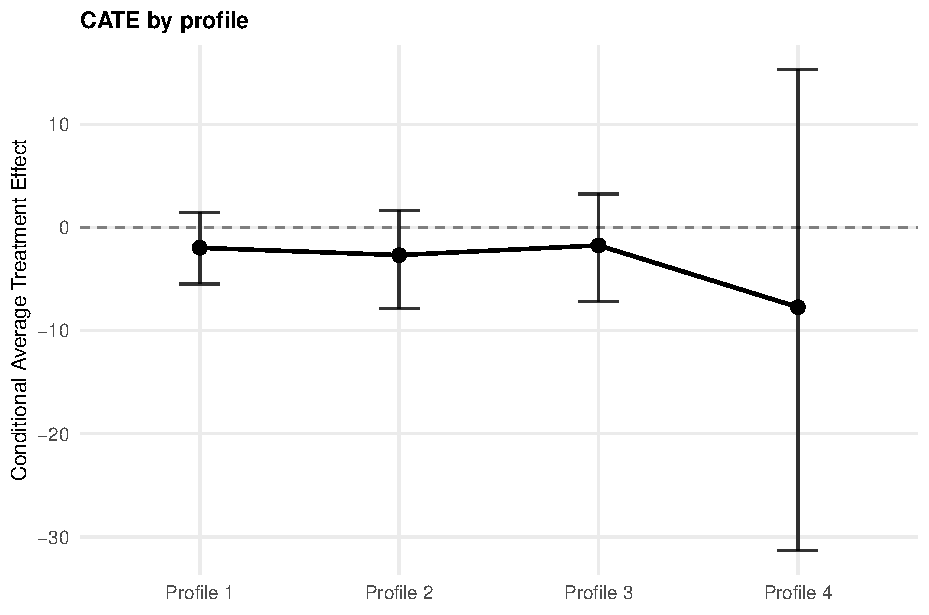
\includegraphics[width=\linewidth]{figure/cate_plot-1} 

}

\caption{Conditional treatment-effect summaries for Lalonde 1978 earnings at the four representative covariate profiles (Profile~1--Profile~4) of Table~\ref{tab:xnew-results}. Left panel: profile-specific conditional average treatment effects $\mathrm{CATE}(x)=\mu_1(x)-\mu_0(x)$ with $95\%$ HPD intervals, returned by \code{cate(fit, newdata = xnew, interval = "hpd")}. Right panel: profile-specific conditional quantile treatment effects $\mathrm{CQTE}(\tau\mid x)=Q_1(\tau\mid x)-Q_0(\tau\mid x)$ at $\tau\in\{0.25,0.50,0.75,0.90,0.95\}$, returned by \code{cqte()}; each cell reports the posterior estimate with the $95\%$ credible interval in brackets.}\label{fig:cate_plot}
\end{figure}

\end{knitrout}

The CQTE estimates reveal heterogeneity across both covariate profiles and quantile levels. At low and median quantile levels, the estimated program effect is close to zero or negative. Uncertainty about treatment effects is high at the upper quantiles, as upper-quantile contrasts rely on fewer observations and are more sensitive to the spliced tail. The analysis provides no evidence of positive program effects; any such effects, if present, appear confined to specific covariate profiles at upper quantiles.

\subsection{Results and interpretation}

Two questions bear on the interpretation: the overall program effect on earnings, and heterogeneity of effects across participant profiles. The first yields no statistically compelling evidence — the average treatment effect is close to zero and the estimated QTE are negative at lower and mid-quantiles. The second yields equivocal findings: treatment effects are profile-specific, and some CQTE at upper quantiles show a positive effect confined to particular subpopulations.

This analysis underscores the value of quantile-based methods for heavy-tailed outcomes. A mean-only analysis provides little evidence of a program effect; the QTE, by contrast, reveals heterogeneity in the treatment effect across the outcome distribution.

\section{Discussion}
\label{sec:discussion}

\pkg{CausalMixGPD} integrates flexible bulk density estimation,
optional EVT-based tail extrapolation, predictor-dependent clustering,
and quantile and density-level causal inference within a single coherent workflow.
The same fitted model supports posterior summaries for densities,
survival curves, analytical means (when they exist), restricted means,
quantiles, and treatment contrasts, thereby obviating the fragmented
analysis pipelines often required when heavy tails and density-level
effects are both of concern.

The package is considerably broader than the spliced examples
emphasized in this article.  Users may work with bulk-only or spliced
models, multiple kernel families on the real line or on positive
support, stick-breaking or CRP backends, and clustering or causal
wrappers built upon the same predictive machinery.  This shared
infrastructure facilitates transitions from exploratory subgroup
analysis to tail-focused prediction and causal reporting without
altering the underlying modeling language.

Several practical limitations warrant acknowledgment.  First,
computation can be demanding.  Mixture models with covariate
dependence, optional tail components, and arm-specific causal fits are
inherently MCMC-intensive, and costs escalate further with sensitivity
analyses, longer chains, or richer predictor sets.

Second, model tuning requires attention.  A spliced analysis inherits
specification choices from both the DPM and peaks-over-threshold
components, including kernel family, truncation level, threshold
specification, and the number of exceedances available for tail
learning.  When overlap is weak or exceedances are sparse, posterior
uncertainty can be substantial; for clustering, the posterior
similarity matrix is often more informative than any single partition
summary.

Third, the current scope is circumscribed.  The causal implementation
is restricted to binary treatments and continuous outcomes under
standard consistency, ignorability, and overlap assumptions.
Propensity-score augmentation can improve covariate adjustment in
observational studies, but it is not a substitute for careful study
design, overlap diagnostics, or sensitivity analysis for unmeasured
confounding.




\bibliography{CausalMixGPD_JSS_refs}


\clearpage
\appendix
\section{Customization of Package and Additional Features}
\label{sec:appendix-features}

This appendix details the customizable features of \pkg{CausalMixGPD}. It covers argument-level customization for model fitting, posterior manipulation, and workflow-specific extensions.

\subsection{Model fitting options and prior specifications}
\label{subsec:app-modeling}

Besides the customizable features illustrated in Sections \ref{subsec:gpd}, \ref{subsec:dpm}, \ref{subsec:causal}, and \ref{subsec:overview-model}, this section lists arguments that allow kernel choice, latent structure, and prior customization alternative to default choices.

\begin{itemize}
\item \textbf{Kernel families and support} (\label{subsec:app-kernels}): the argument \code{kernel} allows to choose among seven different kernel families, defined either with positive support or on the real line. The kernels with positive support are \code{"gamma"}, \code{"lognormal"}, and \code{"invgauss"}; the kernels with real support are \code{"normal"}, \code{"laplace"}, \code{"cauchy"}, and \code{"amoroso"}. The function \code{kernel_support_table()} reports the support, whether the kernel is compatible with GPD, and the supports of the covariates and backend. The function \code{get_kernel_registry()} returns the kernel registry with detailed information such as the parameter names, the default prior mode, and the density/CDF/quantile functions. For causal models, \code{kernel} can be either a single string or a length-two vector specifying different DPM kernels for the two arms. The kernel choice determines the support of the outcome variable and should be made based on the characteristics of the data.

\item \textbf{Backend type and truncation rule} (\label{subsec:app-backends}): the argument \code{backend} determines the structure of the mixing coefficients. The value \code{sb} stands for the stick-breaking scheme while \code{crp} denotes the Chinese Restaurant Process latent allocation scheme. For causal models, \code{backend} can be either a single string or a length-two vector specifying different latent allocation schemes for the two arms. The argument \code{components} sets the maximum number of mixture components (defaulting to the sample size). The argument \code{epsilon} specifies a truncation threshold below which components are dropped and the smallest weight is readjusted. Both arguments can be customized separately for each causal arm.

\item \textbf{Parameter specification and prior setting} (\label{subsec:app-priors}): the argument \code{param_specs} is a named list giving the parameters of the kernel or tail distribution. Each kernel/tail parameter supports three modes: \code{"fixed"}, \code{"dist"}, and \code{"link"}. With \code{"dist"}, the prior can be chosen as any distribution compatible with the parameter and supported by \pkg{nimble}, with hyperparameters specified in the default registry. With \code{"link"}, the kernel/tail parameter is related to the covariates through a linear regression using one of five link functions (\code{"identity"}, \code{"exp"}, \code{"log"}, \code{"softplus"}, or \code{"power"}); the link power is adjusted via \code{link_power} when the last option is selected. With \code{"fixed"}, the parameter is fixed to the constant value specified in \code{param_specs}. For causal models, \code{param_specs} can be either a single named list or a length-two list specifying different parameter specifications for the two arms.
\end{itemize}

\subsection{Fitting, prediction, and posterior output}
\label{subsec:app-fitting}

This section gathers the arguments used after a model class has been chosen: sampler configuration, monitoring, prediction targets, interval summaries, and extraction utilities.

\begin{itemize}
\item \textbf{MCMC configuration} (\label{subsec:app-mcmc}): \code{mcmc} controls \code{niter}, \code{nburnin}, \code{thin}, \code{nchains}, and \code{seed}; causal models split this into \code{mcmc\_outcome} and \code{mcmc\_ps}. Runtime controls include \code{show\_progress}, \code{quiet}, \code{parallel\_chains} with \code{workers}, \code{parallel\_arms} for arm-wise causal fitting, and \code{timing}. CRP-based backends additionally use \code{z\_update\_every} to tune the frequency of global label updates.
\item \textbf{Monitoring and fitting interfaces} (\label{subsec:app-monitors}): \code{monitor = "core"} retains the main structural parameters, whereas \code{"full"} retains all nodes. \code{monitor\_latent = TRUE} stores allocation labels $z_1,\ldots,z_n$, and \code{monitor\_v = TRUE} stores stick-breaking fractions for SB models. Models can be supplied through a formula interface (\code{formula}, \code{data}) or directly through \code{y} and \code{X}; causal fits additionally use \code{treat}. The \code{bundle()} plus \code{mcmc()} workflow separates model construction from sampling when the generated \pkg{nimble} object needs to be inspected or modified first.

\item \textbf{Prediction types and intervals} (\label{subsec:app-predict}): \code{predict()} supports \code{type = "density"}, \code{"survival"}, \code{"quantile"}, \code{"mean"}, \code{"rmean"}, \code{"median"}, \code{"sample"}, and \code{"fit"}. These return posterior summaries of $f(y \mid x)$, $S(y \mid x)$, $Q(\tau \mid x)$, $\mathrm{E}(Y \mid x)$, the restricted mean $\mathrm{E}[\min(Y, c) \mid x]$ via \code{cutoff} and \code{nsim\_mean}, the median (as a special case of the quantile method), posterior predictive draws via \code{nsim}, or retained draw-level fitted values for custom checks. Interval summaries are controlled by \code{interval = "credible"}, \code{"hpd"}, or \code{NULL}, together with \code{level}.

\item \textbf{Summary and extraction methods} (\label{subsec:app-intervals}): \code{summary()} reports posterior means, standard deviations, quantiles, and Effective Sample Size(ESS). \code{params()} reshapes posterior means into component- and coefficient-level layouts; \code{fitted()} and \code{residuals()} provide observation-level predictive summaries.
\item \textbf{Visualization and extraction} (\label{subsec:app-plots}\label{subsec:app-summaries}): \code{plot()} for one-arm fits covers standard MCMC diagnostics, including \code{"traceplot"}, \code{"density"}, \code{"histogram"}, \code{"running"}, \code{"autocorrelation"}, \code{"crosscorrelation"}, \code{"Rhat"}/\code{"grb"}, \code{"effective"}, \code{"geweke"}, \code{"caterpillar"}, \code{"pairs"}, and \code{family = "auto"}. Companion extraction tools include \code{summary()}, \code{params()}, \code{fitted()}, \code{residuals()}, and \code{ess\_summary()}.

\end{itemize}

\subsection{Workflow-specific extensions}
\label{subsec:app-workflows}

This section records controls specific to the clustering and causal workflows in Sections~\ref{subsec:cluster_extension}, \ref{subsec:overview-causal}, \ref{sec:app-clustering}, and \ref{sec:app-causal}. Representative outputs appear in Figures~\ref{fig:app_cluster_overlay}, \ref{fig:app_cluster_test_sizes}, \ref{fig:qte_plot}, and \ref{fig:cate_plot}, with the latter combining the CATE plot and CQTE table.

\begin{itemize}
\item \textbf{Causal estimands} (\label{subsec:app-causal-estimands}): beyond \code{ate()}, \code{qte()}, \code{cate()}, and \code{cqte()}, the package provides \code{att()} for effects averaged over the treated covariate distribution, \code{qtt()} for quantile effects on the treated, and \code{ate\_rmean()} for restricted-mean contrasts. The \code{ate()} and \code{cate()} families also accept \code{type = "mean"} or \code{"rmean"} with a corresponding \code{cutoff}. All effect objects support \code{summary()}, \code{print()}, and \code{plot()} S3 functions. Causal plots route by arm and offer \code{type = "effect"}, \code{"arms"}, or \code{"both"}; QTE plots additionally use \code{facet\_by}; cluster plots provide PSM heatmaps plus label summaries via \code{type = "sizes"}, \code{"certainty"}, and \code{"summary"}. All plots return \pkg{ggplot2} objects and can be converted to \pkg{plotly}.


\item \textbf{Propensity score customization} (\label{subsec:app-ps}): observational causal fits can estimate propensity scores with \code{PS = "logit"}, \code{"probit"}, \code{"naive"}, or \code{FALSE}. The estimated score is appended to the outcome model on either the logit scale (\code{ps\_scale = "logit"}) or probability scale (\code{"prob"}); posterior summaries use \code{ps\_summary = "mean"} or \code{"median"}. Numerical stability is controlled through \code{ps\_clamp}, coefficient shrinkage through \code{ps\_prior}, and the two-stage fitting scheme through separate \code{mcmc\_ps} and \code{mcmc\_outcome} lists.
\item \textbf{Clustering workflow and prediction types} (\label{subsec:app-clustering-details}): \code{dpmix.cluster()} and \code{dpmgpd.cluster()} accept \code{type = "weights"}, \code{"param"}, or \code{"both"} to place predictor dependence in the mixture weights, kernel parameters, or both. Their \code{predict()} methods return either a posterior similarity matrix (\code{type = "psm"}) or representative labels under the Dahl criterion (\code{type = "label"}), including assignments for \code{newdata}. The associated \code{summary()} method reports cluster sizes and within-cluster covariate/response profiles.

\end{itemize}

\subsection{Utilities and Computing Support}
\label{subsec:app-utilities}

The last appendix section includes a selection of helper functions and
resources that accompany the main modeling process.

\begin{itemize}
\item \textbf{Density and quantile utilities} (\label{subsec:app-distutils}): the package provides the complete \textsf{R}-style \code{d}/\code{p}/\code{q}/\code{r} functions for GPD, Inverse Gaussian, Amoroso Distribution with  every supported kernel mixture, and every spliced kernel mixture and GPD distribution. Typical examples include \code{dgpd()}, \code{dgammamix()}, and \code{dgammamixgpd} which are density functions of
the GPD, gamma mixture, and spliced gamma mixture with GPD tail, respectively that can be used directly in modeling and posterior manipulation in \pkg{Nimble}. They are particularly useful for prior checking, generating simulations, benchmarking, and other purposes requiring density and quantile manipulations.

\item \textbf{Simulators and bundled datasets} (\label{subsec:app-simulation}): functions \code{sim\_bulk\_tail()}, \code{sim\_causal\_qte()}, and \code{sim\_survival\_tail()} provide data generation for reproducible benchmarks for bulk and tail and causal analyses; random number generation seeds are supplied by the \code{seed} argument. The package comes bundled with twelve datasets with unconditional/conditional/causal, positive/real-line, and tail/no-tail designs, each featuring outcomes, covariates, treatment indicators where relevant, metadata, and the true values of interest.
\item \textbf{Computational considerations} (\label{subsec:app-computation}): large-scale analyses allow the use of \code{parallel\_chains} with \code{workers}, \code{parallel\_arms} for causal fits, \code{chunk\_size} for predicting in parallel chunks, and \code{ndraws\_pred} for sampling from the posterior predictive distribution of parameters. The \code{show\_progress} and \code{quiet} arguments can be used to control progress reporting and compiler verbosity, respectively, while \code{timing = TRUE} saves time spent on each fit for benchmarking purposes.
\end{itemize}

\end{document}
